\chapter{Tiling the Sky}
\label{chap:tiling}
\chaptoc{}

% ########################################

\newpage
\section{Introduction}
\label{sec:tiling_intro}
\begin{colsection}

In this chapter I describe the software used by GOTO to create an all-sky survey gid, which gravitational wave events are then mapped onto.
%
\begin{itemize}
    \item In \nref{sec:mapping_the_sky} I describe how transient alert localisations are mapped onto the celestial sphere.
    \item In \nref{sec:gototile} I describe the GOTO-tile Python module, and the algorithms is uses to define the all-sky grid and apply skymaps to it.
    \item In \nref{sec:grb_skymaps} I detail how GOTO-tile can be used to create our own skymaps for events that do not use them.
\end{itemize}
%
All work described in this chapter is my own, and has not been published anywhere else. The GOTO-tile module was originally created by Darren White and then expanded by Evert Rol before I took over development.

\end{colsection}

% ########################################

\newpage
\section{Probability skymaps}
\label{sec:mapping_the_sky}
\begin{colsection}

% ~~~~~~~~~~~~~~~~~~~~

\begin{colsection}

\todo{Brief intro, need for a unified way to share sky data}

\end{colsection}

% ~~~~~~~~~~~~~~~~~~~~

\subsection{HEALPix}
\label{sec:healpix}
\begin{colsection}

\gls{healpix} is a system used to define pixelised data on the surface of a sphere~\citep{HEALPix}. Developed at NASA JPL for microwave background data, it is now widely used for other applications including for gravitational wave skymaps produced by the \gls{lvc}. HEALPix divides the sphere into a series of nested (hierarchical) equal-area (although not equal-shape) pixels arranged in declination strips (``isoLatitude''). Shown in \aref{fig:healpix} are the first four orders of spheres, starting from a base resolution with 12 pixels and increasing as each pixel is split into four. The resolution of the sphere is defined using the $N_\text{side}$ parameter, which is given by the number of pixels along the side of one of the 12 base pixels in the given resolution. At every resolution each base-resolution pixel contains $N_\text{side}^2$ pixels, so the total number of pixels in a sphere is given by

\begin{equation}
    N_\text{pix} = 12 N_\text{side}^2.
    \label{eq:healpix_npix}
\end{equation}

Each pixel therefore has an equal area of

\begin{equation}
    \Omega_\text{pix} = \frac{4\pi}{12 N_\text{side}^2} = \frac{\pi}{3 N_\text{side}^2},
    \label{eq:healpix_area}
\end{equation}

on a unit sphere where the radius $r=1$. Taking the celestial sphere, the circumference in degrees is $\SI{360}{\degree} = 2 \pi r$ meaning the area of the whole sky is given by

\begin{equation}
    A_\text{sky} = 4 \pi r^2 = 4 \pi \left ( \frac{\SI{360}{\degree}}{2 \pi} \right )^2 = \frac{129600}{\pi}~\text{sq deg} \approx 41252~\text{sq deg} , %chktex 3
    \label{eq:sky_area}
\end{equation}

and therefore the area of each HEALPix pixel is

\begin{equation}
    A_\text{pix} = \frac{129600}{12 \pi N_\text{side}^2}~\text{sq~deg} \approx \frac{3438}{N_\text{side}^2}~\text{sq~deg}.
    \label{eq:healpix_area_degrees}
\end{equation}

\aref{fig:healpix} shows only the first four orders of HEALPix pixelisation, up to $N_\text{side} = 8$ where the sphere is split into 768 pixels each with an area (which can be considered the resolution of the grid) of 53.7~sq deg. An initial, low-resolution \gls{lvc} skymap might use a grid with $N_\text{side} = 64$ (49 thousand pixels) and resolution (pixel area) of 0.84~sq~deg, where as a final output skymap will have $N_\text{side} = 1024$, 12.5 million pixels and a resolution of $3.27 \times 10^{-3}$~sq~deg (11.7 square arcminutes).

\begin{figure}[t]
    \begin{center}
        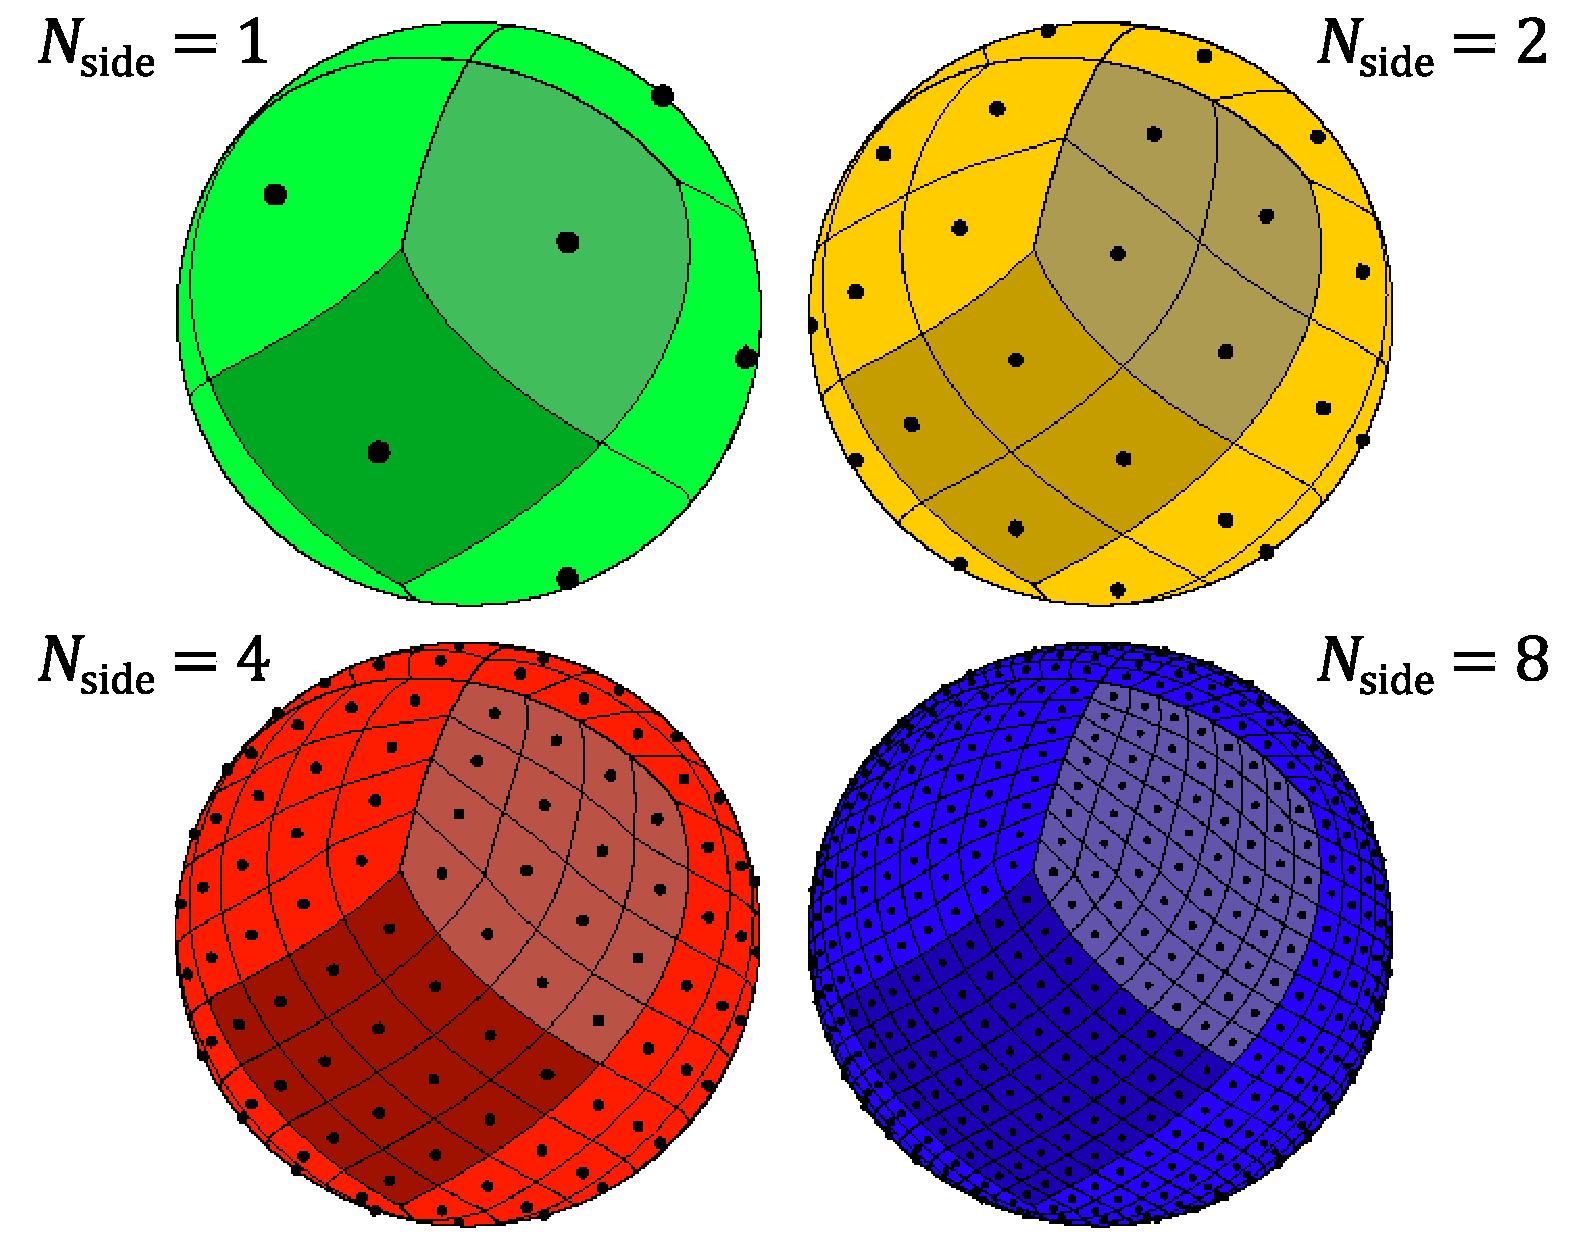
\includegraphics[width=0.7\linewidth]{images/healpix.pdf}
    \end{center}
    \caption[HEALPix partitions of a sphere]{
        HEALPix partitions of a sphere, of increasing order and $N_\text{side}$ resolution parameter. Note that as the resolution increases each pixel on the previous sphere is split into four on the new sphere, and $N_\text{side}$ is the number of pixels along the side of a base-resolution pixel (two of which are highlighted). Adapted (colourised) from Figure~4 of \citet{HEALPix}.
    }\label{fig:healpix}
\end{figure}

In addition to being a way to divide the sphere, each HEALPix pixel has a unique index from one of two different numbering schemes: either the ring (counting around each ring from the north to the south) or nested (based on the sub-pixel tree) system.

\end{colsection}

% ~~~~~~~~~~~~~~~~~~~~

\subsection{Skymaps}
\label{sec:skymaps}
\begin{colsection}

HEALPix is used to provide localisation of sky probabilities for transient astronomical events, in the form of ``skymaps''. Each point on the HEALPix grid is assigned a probability between 0 and 1 that the counterpart object is located within that pixel, and the whole sphere should sum to unity. \aref{fig:skymap_regrade} shows an example \gls{lvc} skymap, for the gravitational wave event S190521r, at various HEALPix $N_\text{side}$ parameters.

As well as the individual probabilities assigned to each pixel, it is also useful to consider the overall spread of the probability. This is done by considering the probability contour areas, typically at the 50\% and 90\% levels. The 50\% contour area of a skymap is defined by encircling the smallest number of pixels so that the total probability within the area is 50\% of the overall skymap probability. When a skymap is defined using GOTO-tile as well as the individual probability values each pixel also has a contour value. This is calculated by sorting all the pixels by probability from highest to lowest, the contour value for each pixel is then cumulative sum of the probability within the pixels above it. This contour value can be considered as the lowest contour area that each pixel is within, meaning the pixels that are contained within the 50\% contour area are those with contour values of less than 50\%. \aref{fig:sim_skymap_probs} and \aref{fig:sim_skymap_conts} illustrate how the contours are calculated for an cartoon 2-dimensional skymap.

\begin{figure}[p]
    \begin{center}
        \begin{tabular}{cc}
            $N_\text{side} = 1$: &
            $N_\text{side} = 2$: \\
            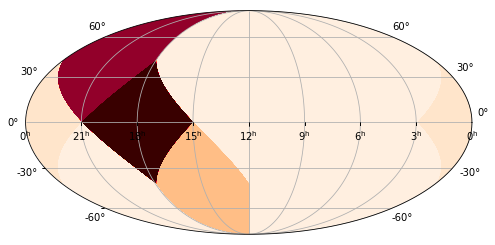
\includegraphics[width=0.45\linewidth]{images/regrade/1.png} &
            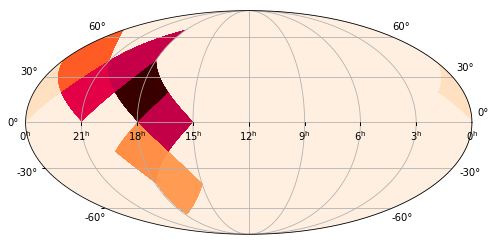
\includegraphics[width=0.45\linewidth]{images/regrade/2.png} \\
            \\
            $N_\text{side} = 4$: &
            $N_\text{side} = 8$: \\
            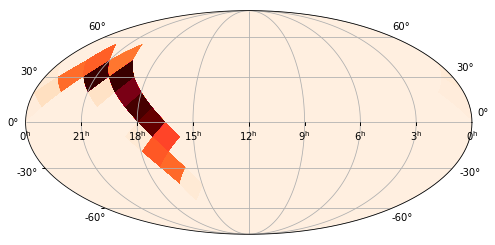
\includegraphics[width=0.45\linewidth]{images/regrade/4.png} &
            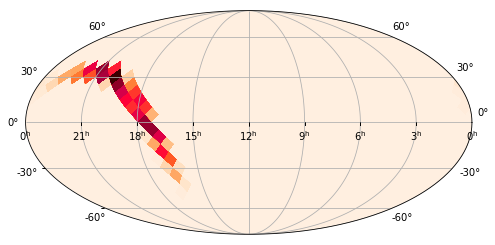
\includegraphics[width=0.45\linewidth]{images/regrade/8.png} \\
            \\
            $N_\text{side} = 16$: &
            $N_\text{side} = 32$: \\
            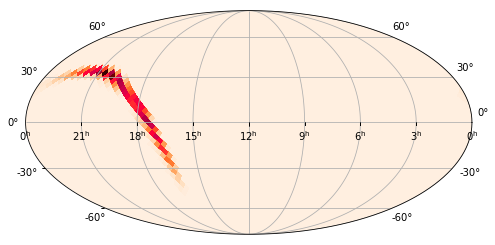
\includegraphics[width=0.45\linewidth]{images/regrade/16.png} &
            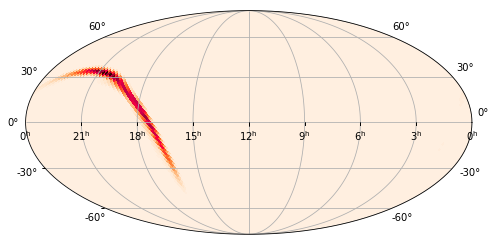
\includegraphics[width=0.45\linewidth]{images/regrade/32.png} \\
            \\
            $N_\text{side} = 64$: &
            $N_\text{side} = 128$: \\
            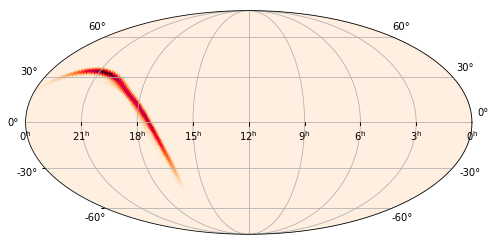
\includegraphics[width=0.45\linewidth]{images/regrade/64.png} &
            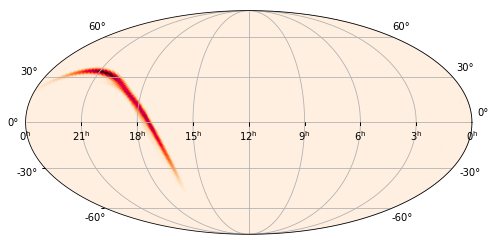
\includegraphics[width=0.45\linewidth]{images/regrade/128.png} \\
        \end{tabular}
    \end{center}
    \caption[Regrading a gravitational wave skymap]{
        Changing the HEALPix resolution of a gravitational wave skymap (also known as regrading). At every stage each pixel is assigned a probability value as shown by the colour scale, which indicates the probability the source is located within that pixel. At lower $N_\text{side}$ individual pixels are visible, but as the resolution increases the structure is less visible.
    }\label{fig:skymap_regrade}
\end{figure}

\begin{figure}[p]
    \begin{center}
        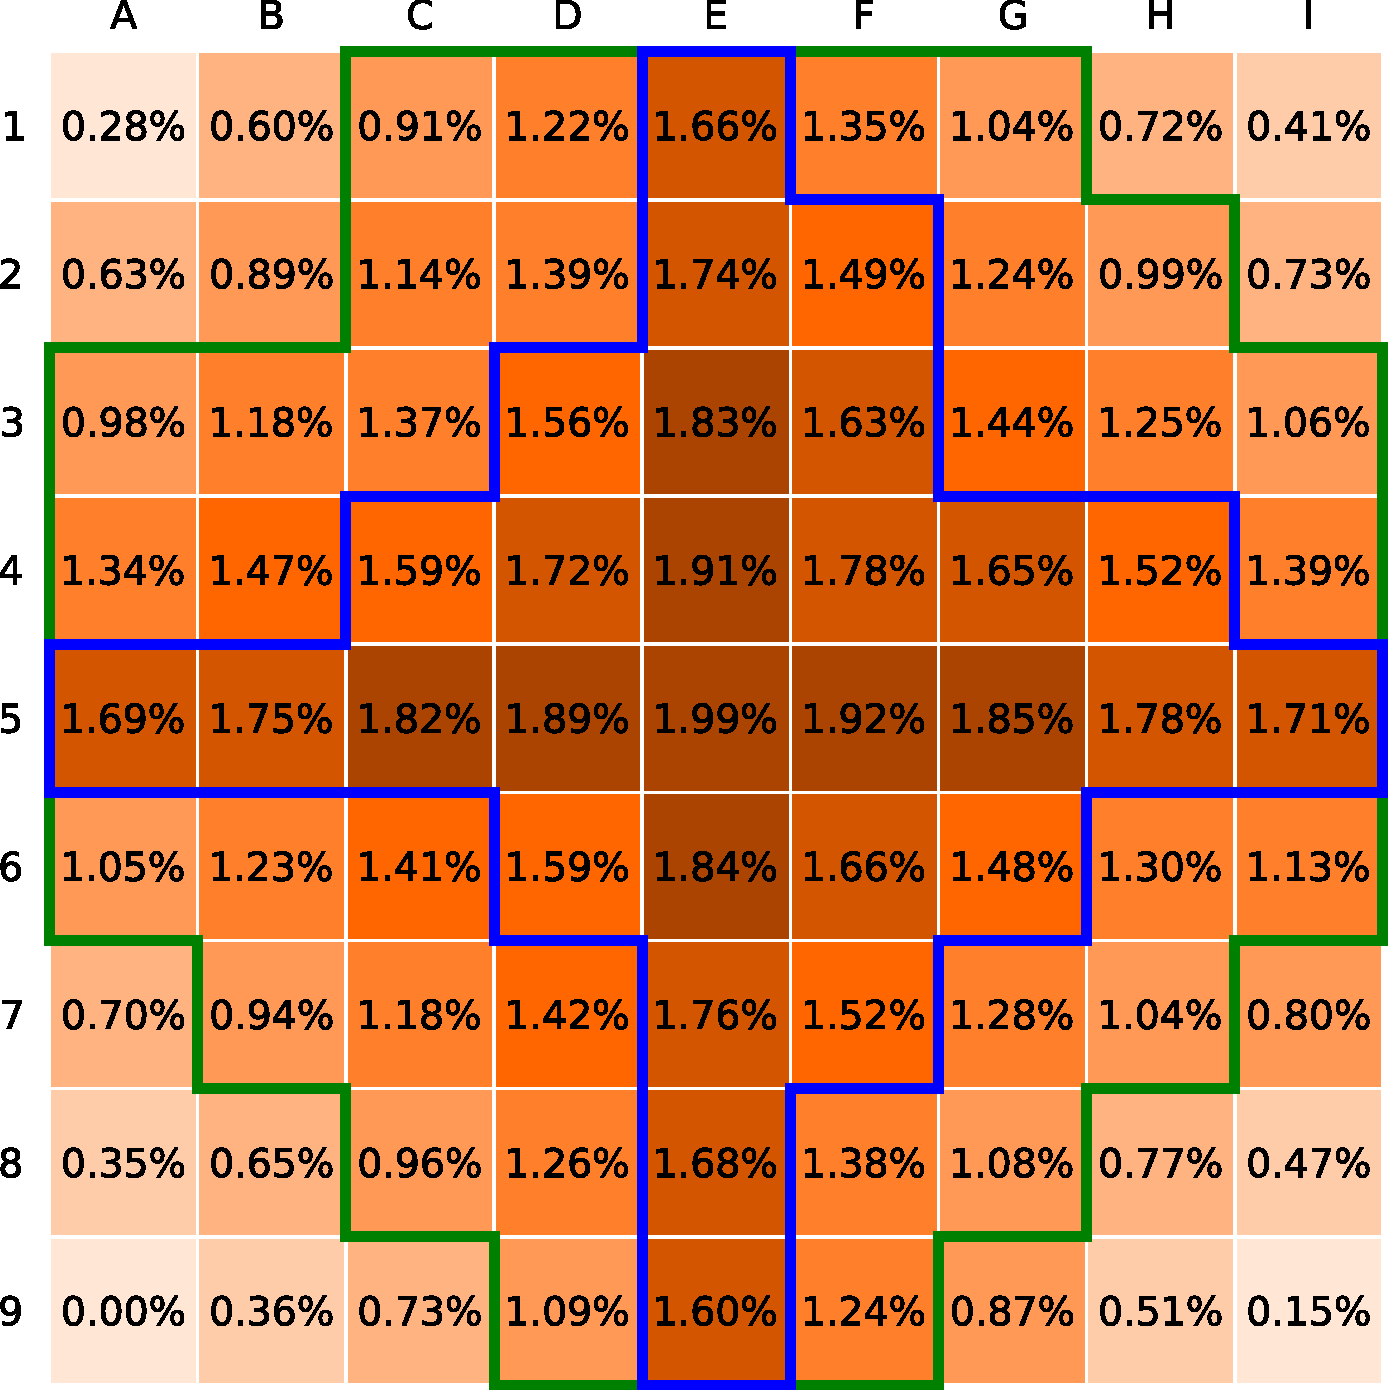
\includegraphics[width=0.95\linewidth]{images/sim/sim_skymap_probs.pdf}
    \end{center}
    \caption[An example 2D probability skymap]{
        A cartoon 2-dimensional skymap. Each pixel (represented by one of the 81 squares) has an assigned probability, and together they all sum to 100\%. The inner blue thick contour line contains 50\% of the probability, while the outer green contour line contains 90\% of the probability. These contours are created based on the values shown in \aref{fig:sim_skymap_conts}.
    }\label{fig:sim_skymap_probs}
\end{figure}

\begin{figure}[p]
    \begin{center}
        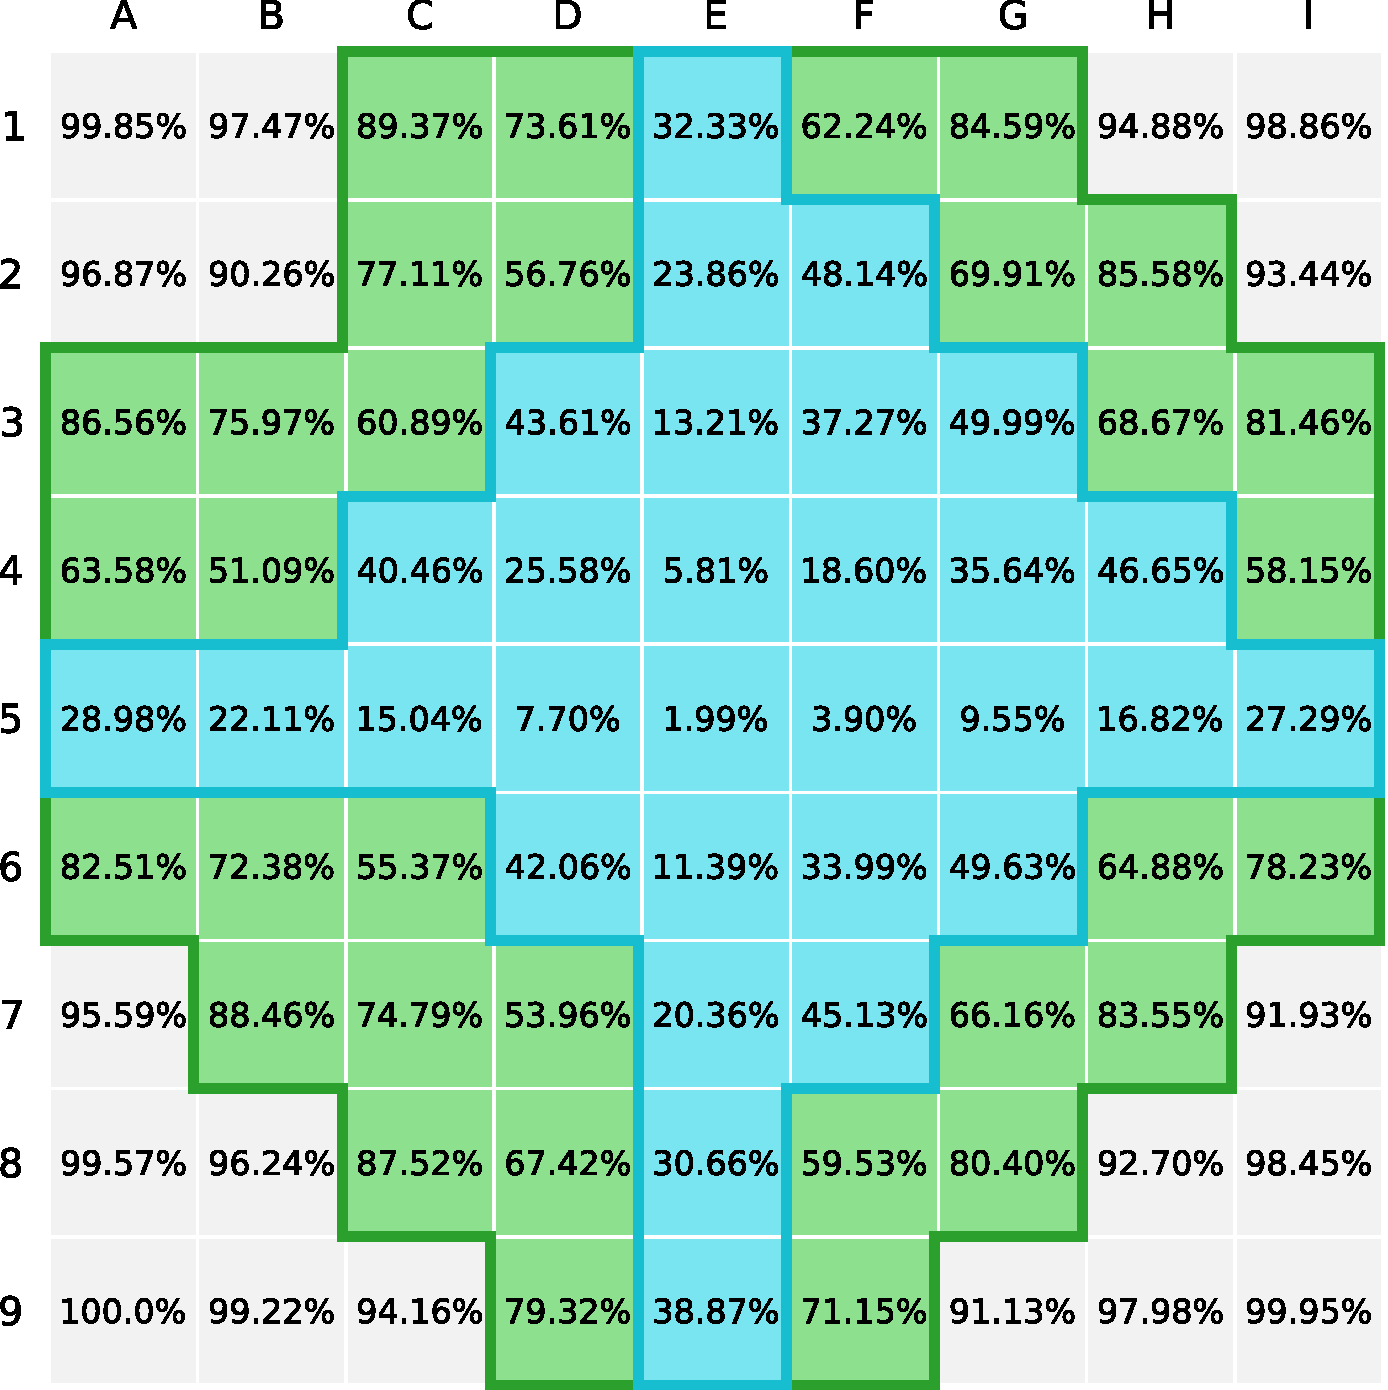
\includegraphics[width=0.95\linewidth]{images/sim/sim_skymap_conts.pdf}
    \end{center}
    \caption[An example 2D skymap with pixel contour values]{
        The same cartoon skymap as in \aref{fig:sim_skymap_probs}, but now each pixel contains its contour value. These are calculated by sorting the pixels by probability and assigning each the value of the cumulative sum. The pixel with the highest probability (E5) has the same contour value as its probability value, the second highest (F5) has the sum of the probability values of both E5 and F5, and this continues to the pixel with the lowest probability value (A9) which has a contour value of 100\%. The thick blue line is the 50\% probability contour, which encloses all pixels with a contour value of less than 50\%. The green line likewise encloses all pixels with a contour value of less than 90\%.
    }\label{fig:sim_skymap_conts}
\end{figure}

\end{colsection}

% ~~~~~~~~~~~~~~~~~~~~

\end{colsection}

% ########################################

\newpage
\section{Defining the sky grid}
\label{sec:gototile}
\begin{colsection}

% ~~~~~~~~~~~~~~~~~~~~

\begin{colsection}

\todo{Needs rewording, define the idea of grids first then GOTO-tile}

GOTO-tile is a \proglang{Python} module (\pkg{gototile} \todo{footnote url?}) created for the \gls{goto} project to contain all the functions and frameworks related to tiling the sky. It was originally developed by Darren White as a way to process \gls{ligo} \gls{gw} skymaps for \gls{goto}, and then maintained by Evert Rol who rearranged it into a module usable for some other telescopes including SuperWASP on La Palma and a proposed southern GOTO node. My contributions to the module have been more fundamental: reworking the foundations to improve how grids are defined and skymaps are applied to them, as well as adding different ways to create skymaps.

\end{colsection}

% ~~~~~~~~~~~~~~~~~~~~

\subsection{Creating sky grids}
\label{sec:grids}
% different ways to make grids
\begin{colsection}

The core of GOTO-tile as it now exists is the \code{SkyGrid} class. This is used to define a sky grid, a collection of `tiles' defined as points on the celestial sphere (\aref{fig:sphere}). These tiles are aligned to the celestial right ascension/declination coordinates, and are designed to create a base framework for observations to be mapped to.

The most important parameter required when defining a sky grid is the field of view of the telescope, which is taken as the size of the tiles that make up the grid. This is defined by giving a width and height value in degrees, meaning the tiles can only be square or rectangular. This is typically fine for the \gls{goto} array, although there was a period when having three \glspl{ut} in an `L'-shape was considered. This was abandoned due mainly to the complexity of tiling the grid based on abstract shapes.

The second parameter required to define a sky grid is the desired overlap between the tiles. This is given as a value between zero and one in both the right ascension and declination directions, with zero meaning no overlap and one meaning all the tiles are completely overlapping (as this would lead to infinite tiles being created in practice the overlap is restricted to no more than $0.9$). This is used to define the spacing between the tile centrers, although exactly how depends on the algorithm used.

As GOTO-tile has been developed the algorithm used to define tile centres has evolved and improved, but the basic method has remained the same:

\begin{enumerate}
    \item Define equally spaced lines of constant declination, separated by the value $\Delta\delta$ (\aref{fig:deltadelta}). These lines are the basis for the grid, which is defined in ``strips'' of tiles. Exactly how $\Delta\delta$ is defined based on the field of view and overlap parameters depends on the algorithm, in particular how to deal with the poles in case $\Delta\delta$ is not a factor of \SI{90}{\degree}.
    \item Once the strips are defined, then each is filled equally spaced points separated by the value $\Delta\alpha$ (\aref{fig:deltaalpha}). This value is constant for each strip but is (in most algorithms) a function of declination ($\Delta\alpha(\delta)$), meaning that moving away from the equator to the poles each strip will contain a reducing number of points.
    \item These points are then defined as the centre of the tiles, the size of which is given by the field of view (\aref{fig:tiledsphere}).
\end{enumerate}

Once the grid has been created it is encapsulated within the GOTO-tile \code{SkyGrid} class. Each tile is defined by a coordinate at its centre, and each is also given a unique name of the form \code{`T0001'}. The grid itself is also given a name formed using the input field of view and overlap parameters, so a grid created with a field of view of \SI{3.7}{\degree}$\times$\SI{4.9}{\degree} and overlap factor of 0.1 (this is the grid used for the \gls{goto} 4-\gls{ut} all-sky survey) is given the name \code{`allsky-3.7x4.9--0.1--0.1'}. In this way a given tile in a given grid can be recreated just from the names, which is used when storing the grid and tile details in the observation database (see \aref{sec:obsdb}). % chktex 29

% ---------

\begin{figure}[p]
    \begin{center}
        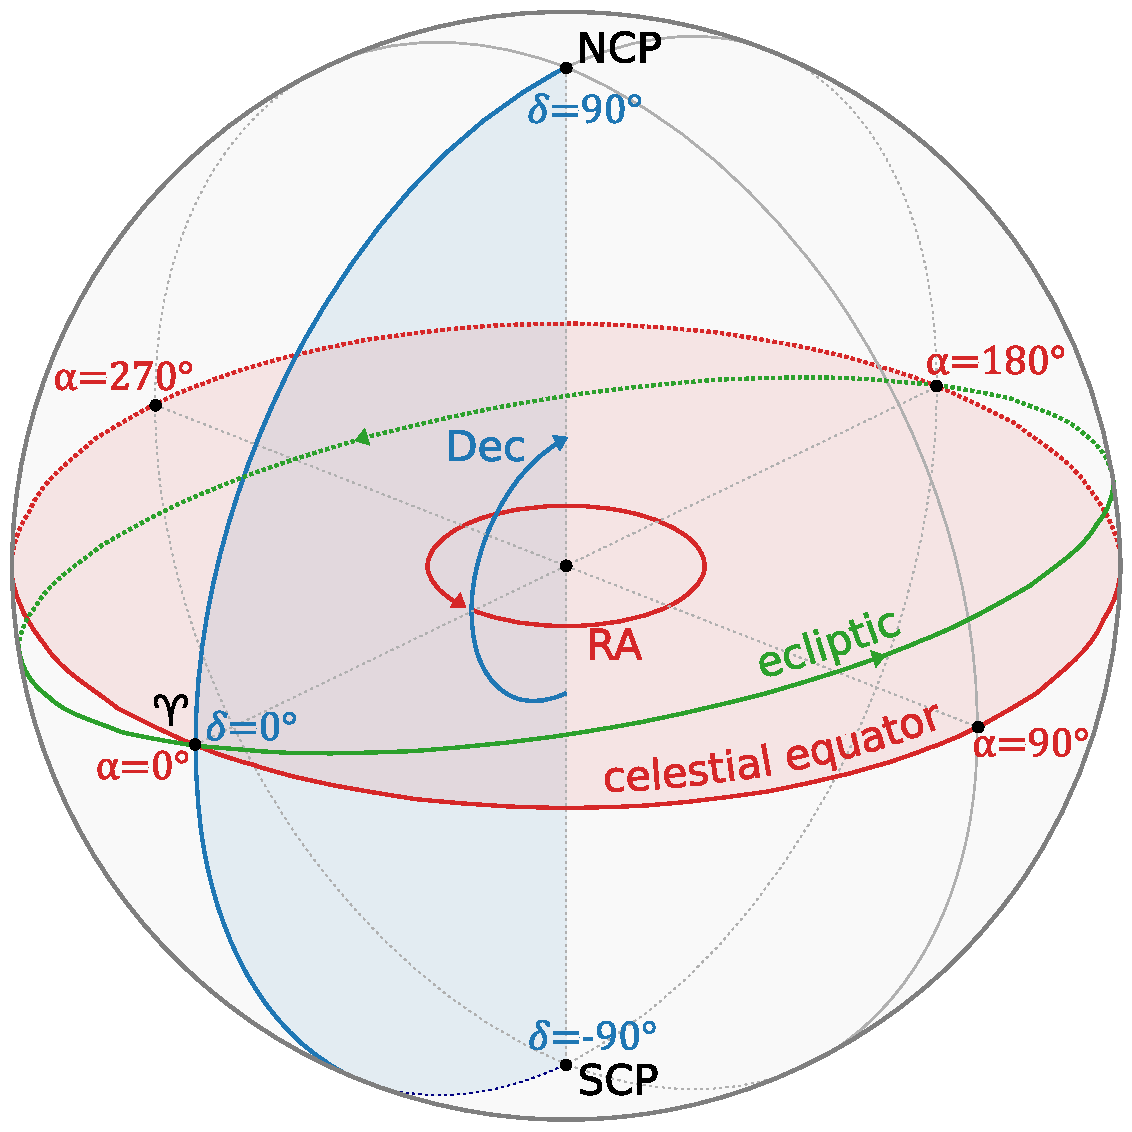
\includegraphics[width=\linewidth]{images/globe1.pdf} %TODO:recolour
    \end{center}
    \caption[The celestial sphere]{
        The celestial sphere. The celestial equator is marked in \textcolorbf{Red}{red}, the vernal equinox (where the ecliptic (not shown) crosses the equator) is marked with the symbol \Aries{} and the meridian that intercepts the vernal equinox is marked in \textcolorbf{NavyBlue}{blue}. The northern and southern celestial poles are marked as NCP and SCP respectively. The definition of the equatorial coordinate system is shown: declination (Dec, $\delta$) is defined as the angle from the equator, ranging from \SI{-90}{\degree} at the SCP to \SI{90}{\degree} at the NCP, and right ascension (RA, $\alpha$) is defined as angle east from the vernal equinox between \SI{0}{\degree} and \SI{360}{\degree}.
    }\label{fig:sphere}
\end{figure}

\begin{figure}[p]
    \begin{center}
        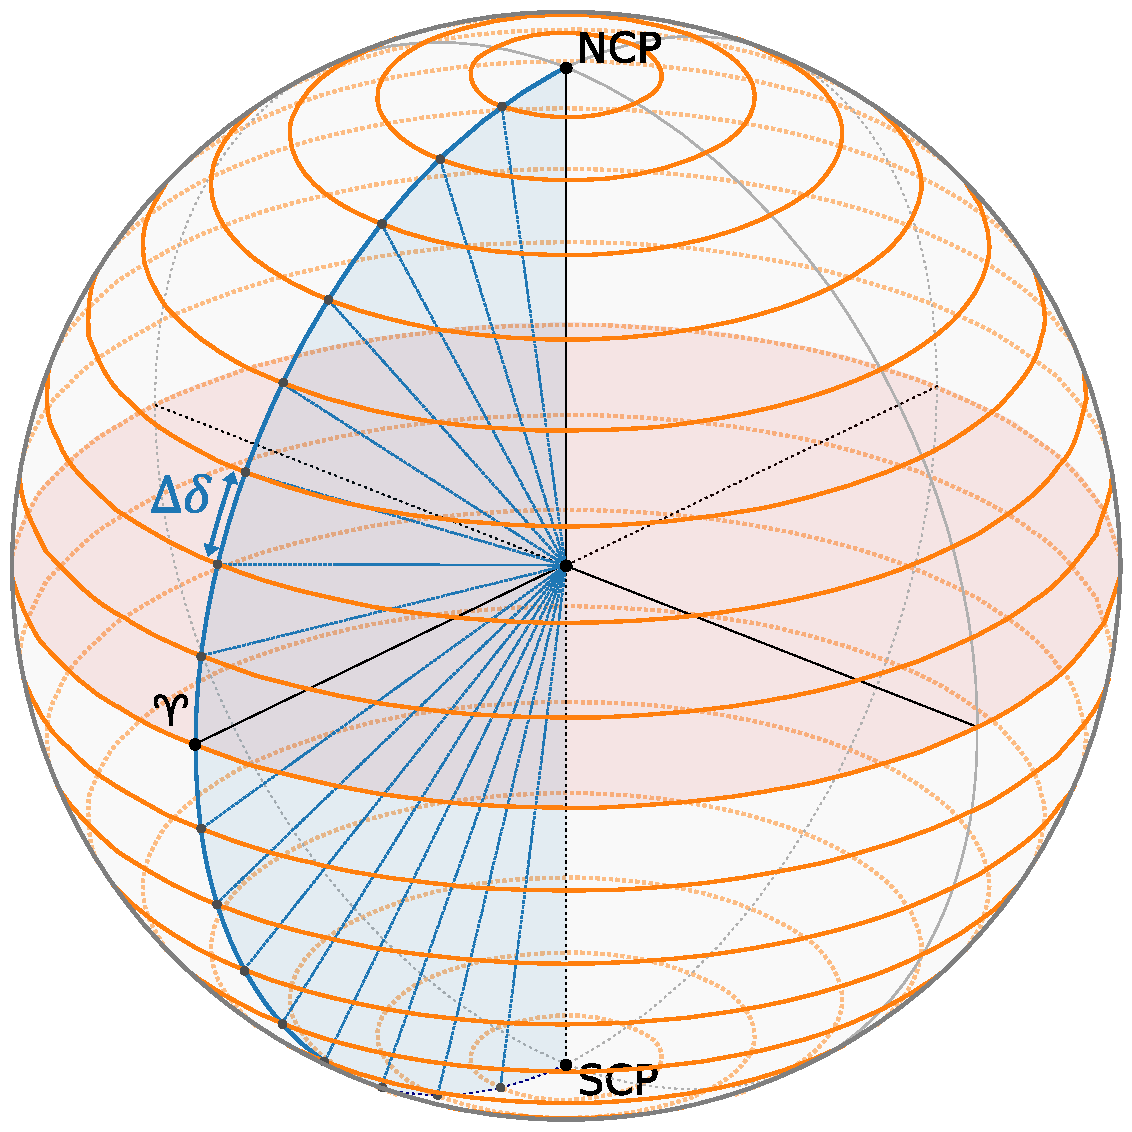
\includegraphics[width=\linewidth]{images/globe2.pdf}
    \end{center}
    \caption[Defining declination strips]{
        The first stage when creating a sky grid is defining the declination strips. This is done by dividing the full range of declination (\SI{-90}{\degree} to \SI{90}{\degree}) equally by a constant spacing value $\Delta\delta$. In this example $\Delta\delta =$ \SI{10}{\degree}, and so strips are defined at $\delta=$ \SI{0}{\degree}, \SI{10}{\degree}, \SI{20}{\degree} etc\ldots, and mirrored in the southern hemisphere. There is always a strip with $\delta=0$. Exactly how the strips are defined when $\Delta\delta$ is not an integer factor of \SI{90}{\degree} depends on the algorithm used, in this case using the ``minverlap'' algorithm the strips range from \SI{-90}{\degree} to \SI{90}{\degree} and include a ``strip'' at the poles which will contain single tile (as shown in \aref{fig:tiledsphere}).
    }\label{fig:deltadelta}
\end{figure}

\begin{figure}[p]
    \begin{center}
        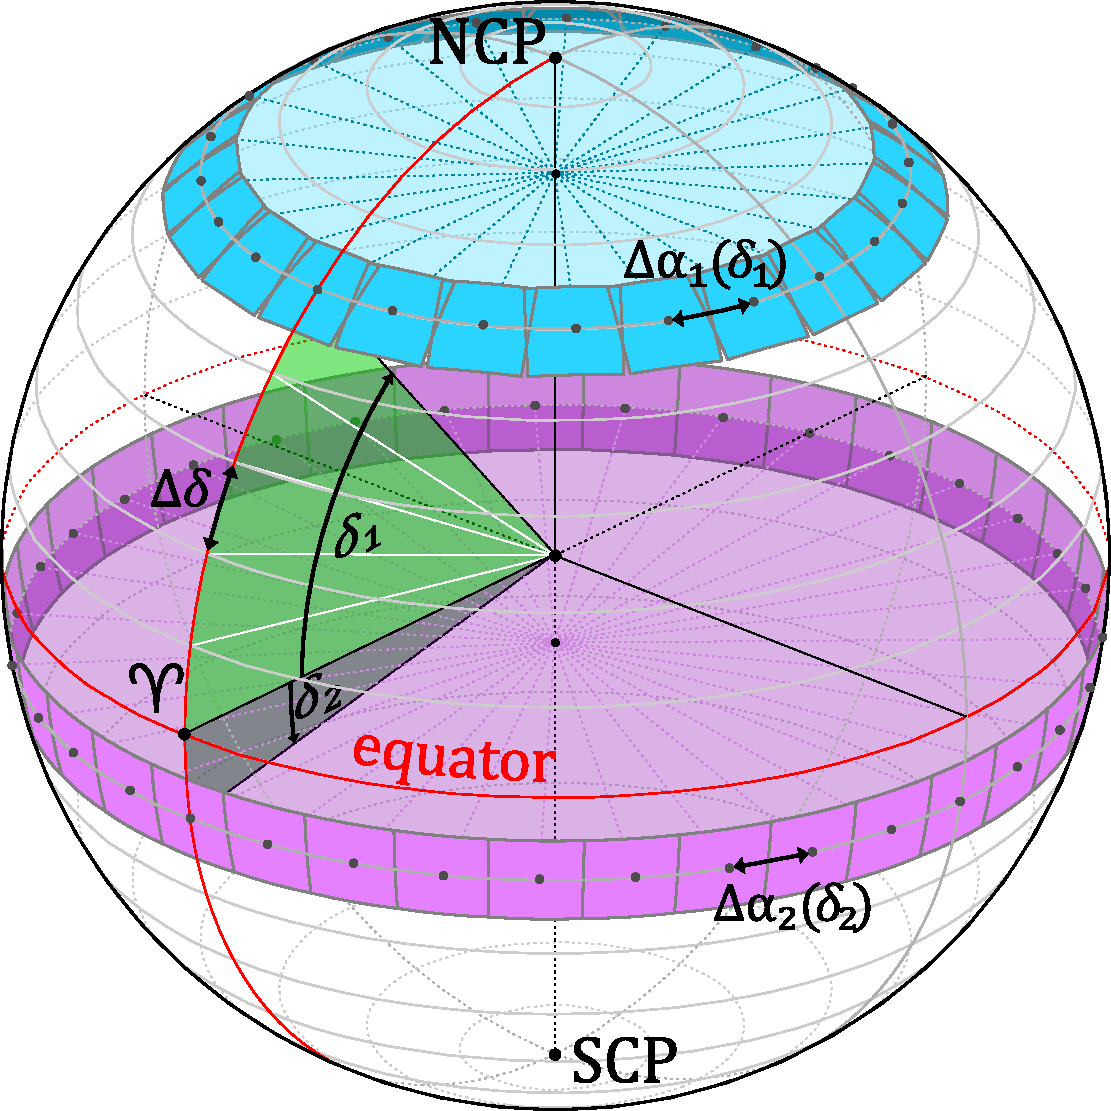
\includegraphics[width=\linewidth]{images/globe3.pdf}
    \end{center}
    \caption[Defining the spacing between tiles]{
        After the declination strips are defined (see \aref{fig:deltadelta}) for each strip tile centres are defined with a set spacing $\Delta\alpha(\delta)$. Unlike $\Delta\delta$, which is fixed across the sphere, $\Delta\alpha$ varies as a function of declination meaning strips closer to the poles will contain fewer tiles. Two examples of defining tiles are shown above, one at declination $\delta_1$ (\SI{50}{\degree}, in \textcolorbf{BlueGreen}{cyan}) in the northern hemisphere and another at $\delta_2$ (\SI{-10}{\degree}, in \textcolorbf{Purple}{purple}) in the southern hemisphere. The results of the ``minverlap'' algorithm are shown, previous algorithms had different ways of defining $\Delta\alpha$ that would have resulted in different spacings.
    }\label{fig:deltaalpha}
\end{figure}

\begin{figure}[p]
    \begin{center}
        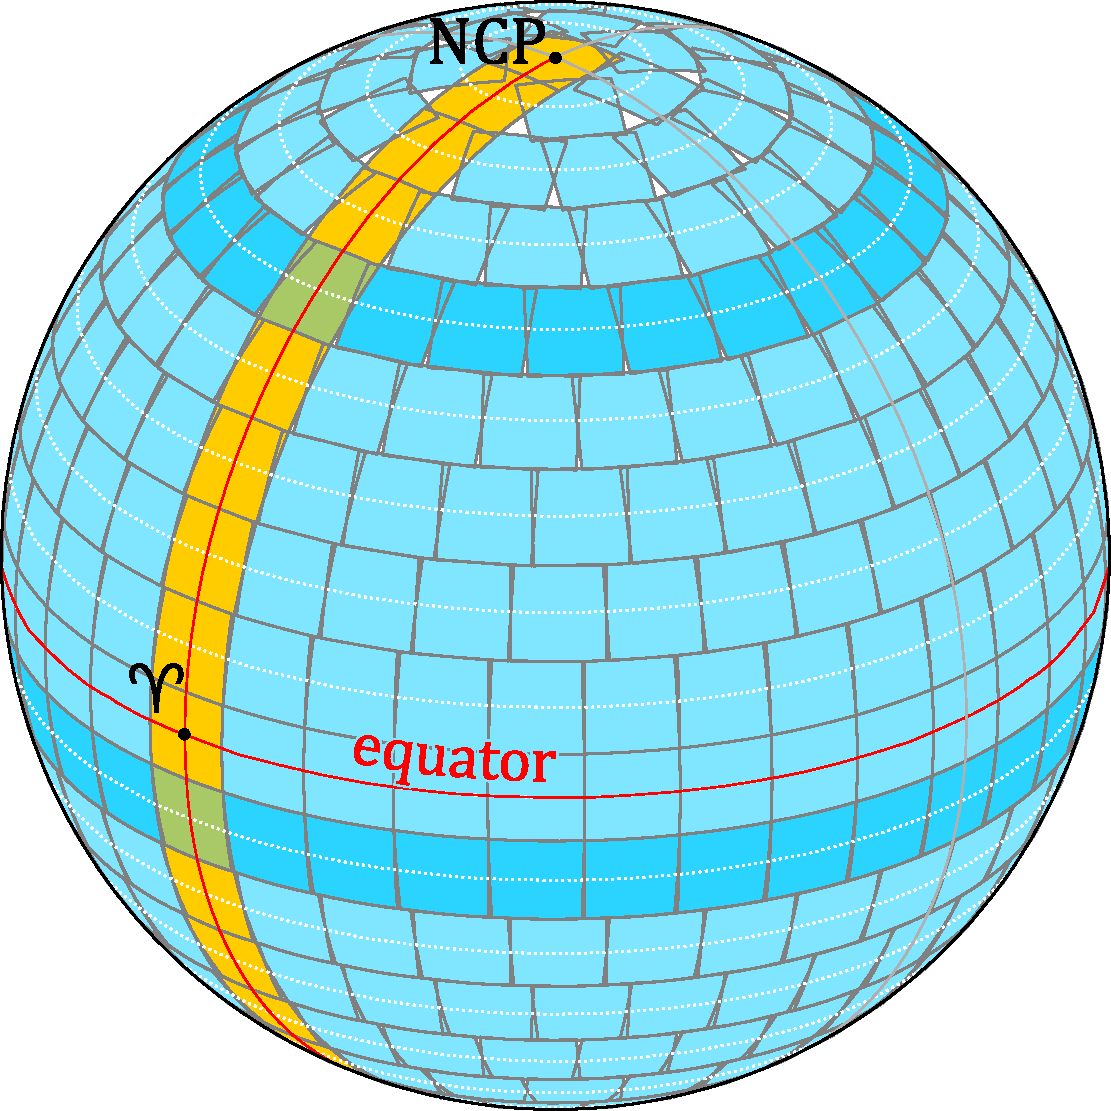
\includegraphics[width=\linewidth]{images/globe4.pdf}
    \end{center}
    \caption[A fully tiled sphere]{
        Once every declination strip is complete the full grid is defined, as shown above. The same two strips are shown in \textcolorbf{BlueGreen}{cyan} and \textcolorbf{Purple}{purple} as in \aref{fig:deltaalpha}. Due to each strip starting the tile spacing at RA$=0$, there is a fully aligned column of tiles along the vernal equinox, shown in \textcolorbf{Orange}{orange}. The grid in these examples was defined using the ``minverlap'' algorithm, with each tile having a field of view of \SI{10}{\degree} $\times$ \SI{10}{\degree} and the overlap was set to zero for clarity (note this can lead to gaps between tiles towards the poles, as visible here). In this case the complete grid contains 424 tiles.
    }\label{fig:tiledsphere}
\end{figure}

\newpage

\end{colsection}

% ~~~~~~~~~~~~~~~~~~~~

\subsection{Defining gridding algorithms}
\label{sec:algorithms}
\begin{colsection}

There have been three primary algorithms defined in GOTO-tile's history.

% ---------
\subsubsection{The product algorithm}

The first has since retroactively been called the ``\textbf{product}'' algorithm, and was used when Darren White first wrote GOTO-tile. It first defines the declination step size as

\begin{equation}
    \Delta\delta = f_\text{dec}(1-v_\text{dec}),
    \label{eq:product_deltadelta}
\end{equation}

where $f_\text{dec}$ and $v_\text{dec}$ are respectively the field of view and overlap parameters in the declination direction. The declination strips are then defined by taking steps of this size from the equator towards the poles, stopping when $|\delta| > 90$. The equivalent formula is used to calculate the steps in right ascension

\begin{equation}
    \Delta\alpha = f_\text{RA}(1-v_\text{RA}).
    \label{eq:product_deltaalpha}
\end{equation}

The clear downside of this method is that $\Delta\alpha$ does not vary depending on declination. In effect this algorithm attempts to define the grid as if it was on a flat plane, where the tiles could be arranged in orthogonal rows and columns. In practice when applied to a sphere this leads to a vast number of redundant tiles at the poles, as shown in \aref{fig:product}.

% ---------
\subsubsection{The cosine algorithm}

Due to the obvious problems with the previous algorithm a replacement was written by Evert Rol, which I have since called the ``\textbf{cosine}'' algorithm. It is a more refined version of the ``product'' algorithm, and the declination strips are calculated in the same manor using \aref{eq:product_deltadelta}. However \aref{eq:product_deltaalpha} is modified to depend on declination into

\begin{equation}
    \Delta\alpha(\delta) = \frac{f_\text{RA}(1-v_\text{RA})}{\cos(\delta)}.
    \label{eq:cosine_deltaalpha}
\end{equation}

This produces a much more sensible grid as shown in \aref{fig:cosine}. However there remained an issue of asymmetry: the strips are arranged increasing and decreasing from $\delta=0$ and the tiles are then arranged within the strips starting from $\alpha=0$. As visible in \aref{fig:cosine} this leads to varying overlaps when the the tiles within the strips overlap as $\alpha$ approaches \SI{360}{\degree}. Although more subtle there are similar issues at the north and south poles, and it's common for there to be small gaps between the tiles at high and low declinations.

% ---------
\subsubsection{The minverlap algorithm}

Due to these problems I created a new method to create the grid, called the ``\textbf{minverlap}'' (minimum overlap) algorithm. The same grid created with this algorithm is shown in \aref{fig:minverlap}. The intention of the new algorithm was to solve these issues by adjusting the spacing between tiles to prevent odd gaps. The previous two algorithms both treat the given overlap parameter as as unegotiable, and if the resulting spacings don't give an integer number of tiles within the ranges available then there are uneven gaps at the edges. This is shown more clearly in \aref{fig:cosine_spacing}, where a tricky spacing results in gaps at the poles and variable overlaps on the meridian. The ``minverlap'' algorithm solves this by treating the given overlap parameter not as fixed but as the \textit{minimum} required overlap between tiles. If a grid is requested with an overlap of $0.2$ (20\%), but the odd field of view of the tiles doesn't fit neatly into the ranges then the overlap can be incensed until the tiles fit.

In order to do this mathematically, it is first necessary to find the number of tiles $n$ that would fit into the range using the previous spacing, and then if it isn't an integer number round it up to the next whole number. In declination this is calculated as

\begin{equation}
    n_\text{dec} = \left \lceil \frac{90}{f_\text{dec}(1-v_\text{dec})} \right \rceil,
    \label{eq:minverlap_ndec}
\end{equation}

where $\lceil x \rceil$ is the mathematical ceiling function. This is a modification of the previous \aref{eq:product_deltadelta} but one that will always find an integer number of tiles. For example, with $f_\text{dec} = $ \SI{13}{\degree} and $v_\text{dec} = 0.2$ the previous spacing $\Delta\delta = 13 \times (1-0.2) = $ \SI{10.4}{\degree}. This clearly doesn't divide into the \SI{90}{\degree} range without a remainder, which is \SI{6.8}{\degree} as shown in \aref{fig:cosine_spacing}. The problem is that \SI{90}{\degree} $/$ \SI{10.4}{\degree} $= 8.65$. So the previous algorithms will fit in 8 tiles and have over half a tile remaining at the poles. Instead the minverlap algorithm rounds this up to $n_\text{dec} = 9$ tiles, and then simply calculates the spacing using

\begin{equation}
    \Delta\delta = \frac{90}{n_\text{dec}}.
    \label{eq:minverlap_deltadelta}
\end{equation}

In this case the new $\Delta\delta = $ \SI{10}{\degree}, which gives an even arrangement of tiles from the equator to the poles, as shown in \aref{fig:minverlap_spacing}. The other benefit of this method is that, in addition to there always being a declination strip at $\delta=0$, there will always be ``strips'' at \SI{+90}{\degree} and \SI{-90}{\degree}, which results in a single tile being located covering the poles and ensuring there are no major gaps in coverage.

Right ascension is treated similarly. The integer number of tiles that can fit into a given declination strip is given by

\begin{equation}
    n_\text{RA}(\delta) = \left \lceil \frac{360}{f_\text{RA}(1-v_\text{RA})/\cos(\delta)} \right \rceil + 1,
    \label{eq:minverlap_nra}
\end{equation}

where the $+1$ is here necessary to account for tiles being located both at $\alpha=$\SI{0}{\degree} and $\alpha=$\SI{360}{\degree}. The logic is exactly the same as with declination, and the revised spacing is given by

\begin{equation}
    \Delta\alpha(\delta) = \frac{360}{n_\text{RA}(\delta)}.
    \label{eq:minverlap_deltaalpha}
\end{equation}

The effect of this is also shown in \aref{fig:minverlap_spacing}, and tiles are uniformly spaced around the declination strip. Note here the ceiling function does produce a slight degeneracy in $\Delta\alpha$ being a function of $\delta$. Using the same parameters as the previous example $\Delta\delta=$\SI{10}{\degree}, so declination strips start at \SI{0}{\degree} and continue to \SI{\pm10}{\degree}, \SI{\pm20}{\degree} \ldots (mirrored in both hemispheres). From \aref{eq:minverlap_nra} the number of tiles on the equator is $n_\text{RA}(\delta=\SI{0}{\degree}) = \lceil 360/(10.4/\cos(0)) \rceil + 1 = \lceil 34.6 \rceil + 1 = 36$. But on the next strip up (or down) $n_\text{RA}(\delta=\SI{\pm10}{\degree}) = \lceil 360/(10.4/\cos(\pm10)) \rceil + 1 = \lceil 34.1 \rceil + 1 = 36$ as well. This is a natural occurrence as there are only a limited number of ways to fit an integer number of fixed tiles into a given range, and so as shown in \aref{fig:minverlap} the three strips around the equator align perfectly with the same number of tiles.

% ---------
\subsubsection{Limitations of the minverlap algorithm}

The new ``minverlap'' algorithm is an improvement on the previous versions, in particular as it reduces the occurrences of gaps in coverage closer to the poles that happened when using the ``cosine'' algorithm. However the new algorithm is not perfect and gaps can still occur if the starting overlap parameter is very low. For example, \aref{fig:tiledsphere} shows a sphere tiled using the ``minverlap'' algorithm and an overlap parameter of 0. In this case gaps are visible in the strips of tiles just below the northern celestial pole. A proposed solution to this problem would be to force tiles to meet at their lower corners (in the northern hemisphere, upper corners in the south), therefore overlapping further and removing the possibility of gaps forming due to the angle between the tiles. An attempt to make this change and create an ``enhanced minverlap'' algorithm was tested, however ultimately it proved unnecessary. Although the current algorithm is deficient at low overlap values, this is only an issue for large tiles and very low overlaps. The \SI{10}{\degree} $\times$ \SI{10}{\degree} tiles and 0\% overlap used for \aref{fig:tiledsphere} are extreme values, and even for the roughly \SI{8}{\degree} $\times$ \SI{5}{\degree} full field of view of a full GOTO telescope the overlap has to be less than 10\% before noticeable gaps start appearing. As well, from the site on La Palma the northern celestial pole is actually below \glspl{goto} nominal horizon of \SI{30}{\degree}, therefore meaning tiles close to the pole will never be visible and the gaps in coverage were irrelevant. Should GOTO-tile be applied in the future to other projects then this issue would need to be revisited, but it was not a priority to fix within the context of this work.

\newpage

\begin{figure}[p]
    \begin{minipage}[c]{0.46\textwidth}
        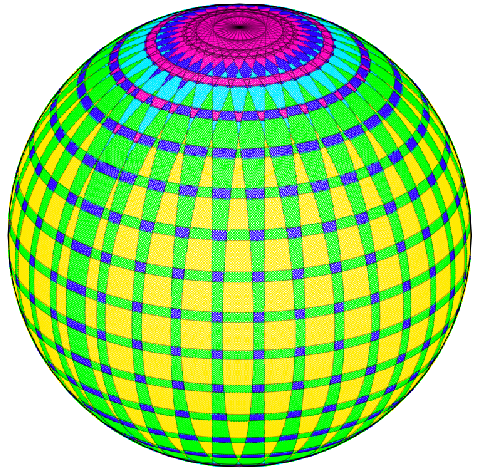
\includegraphics[width=\linewidth]{images/algo_product.pdf}
    \end{minipage}
    \hfill
    \begin{minipage}[c]{0.50\textwidth}
        \caption[The ``product'' gridding algorithm]{
            A sky grid of tiles defined using the ``product'' gridding algorithm. The inputs were a field of view of \SI{13}{\degree} $\times$ \SI{13}{\degree} and an overlap factor of $0.2$ in both axes. The colours show overlapping coverage: \textcolorbf{Yellow}{yellow} areas are within only one tile, \textcolorbf{green}{green} two, \textcolorbf{blue}{blue} three, \textcolorbf{cyan}{cyan} four and \textcolorbf{RubineRed}{pink} five or more. This grid contains 595 tiles. Note the constant spacing of tiles in RA and the huge number of redundant tiles at the pole.
        }\label{fig:product}
    \end{minipage}
\end{figure}

\begin{figure}[p]
    \begin{minipage}[c]{0.50\textwidth}
        \caption[The ``cosine'' gridding algorithm]{
            A sky grid of tiles defined using the ``product'' gridding algorithm. The input parameters and colours are the same as in \aref{fig:product}. This grid contains 393 tiles. Note the asymmetric ``seam'' along the $\alpha=0$ meridian, and the \textcolorbf{red}{red} areas near the pole that are not within the area of any tiles.
        }\label{fig:cosine}
    \end{minipage}
    \hfill
    \begin{minipage}[c]{0.46\textwidth}
        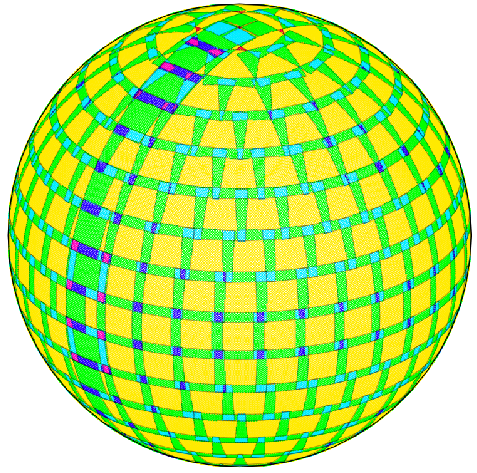
\includegraphics[width=\linewidth]{images/algo_cosine.pdf}
    \end{minipage}
\end{figure}

\begin{figure}[p]
    \begin{minipage}[c]{0.46\textwidth}
        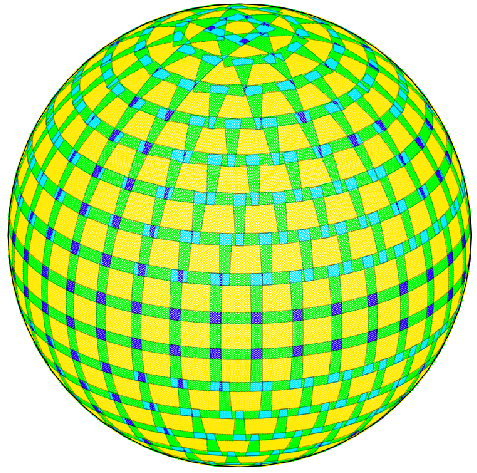
\includegraphics[width=\linewidth]{images/algo_minverlap.pdf}
    \end{minipage}
    \hfill
    \begin{minipage}[c]{0.50\textwidth}
        \caption[The ``minverlap'' gridding algorithm]{
            A sky grid of tiles defined using the ``minverlap'' gridding algorithm. The input parameters and colours are the same as in \aref{fig:product}. This grid contains 407 tiles.  Note the even spacing of tiles even over the $\alpha=0$ meridian, and the better coverage at the pole.
        }\label{fig:minverlap}
    \end{minipage}
\end{figure}

\newpage

\begin{figure}[p]
    \begin{center}
        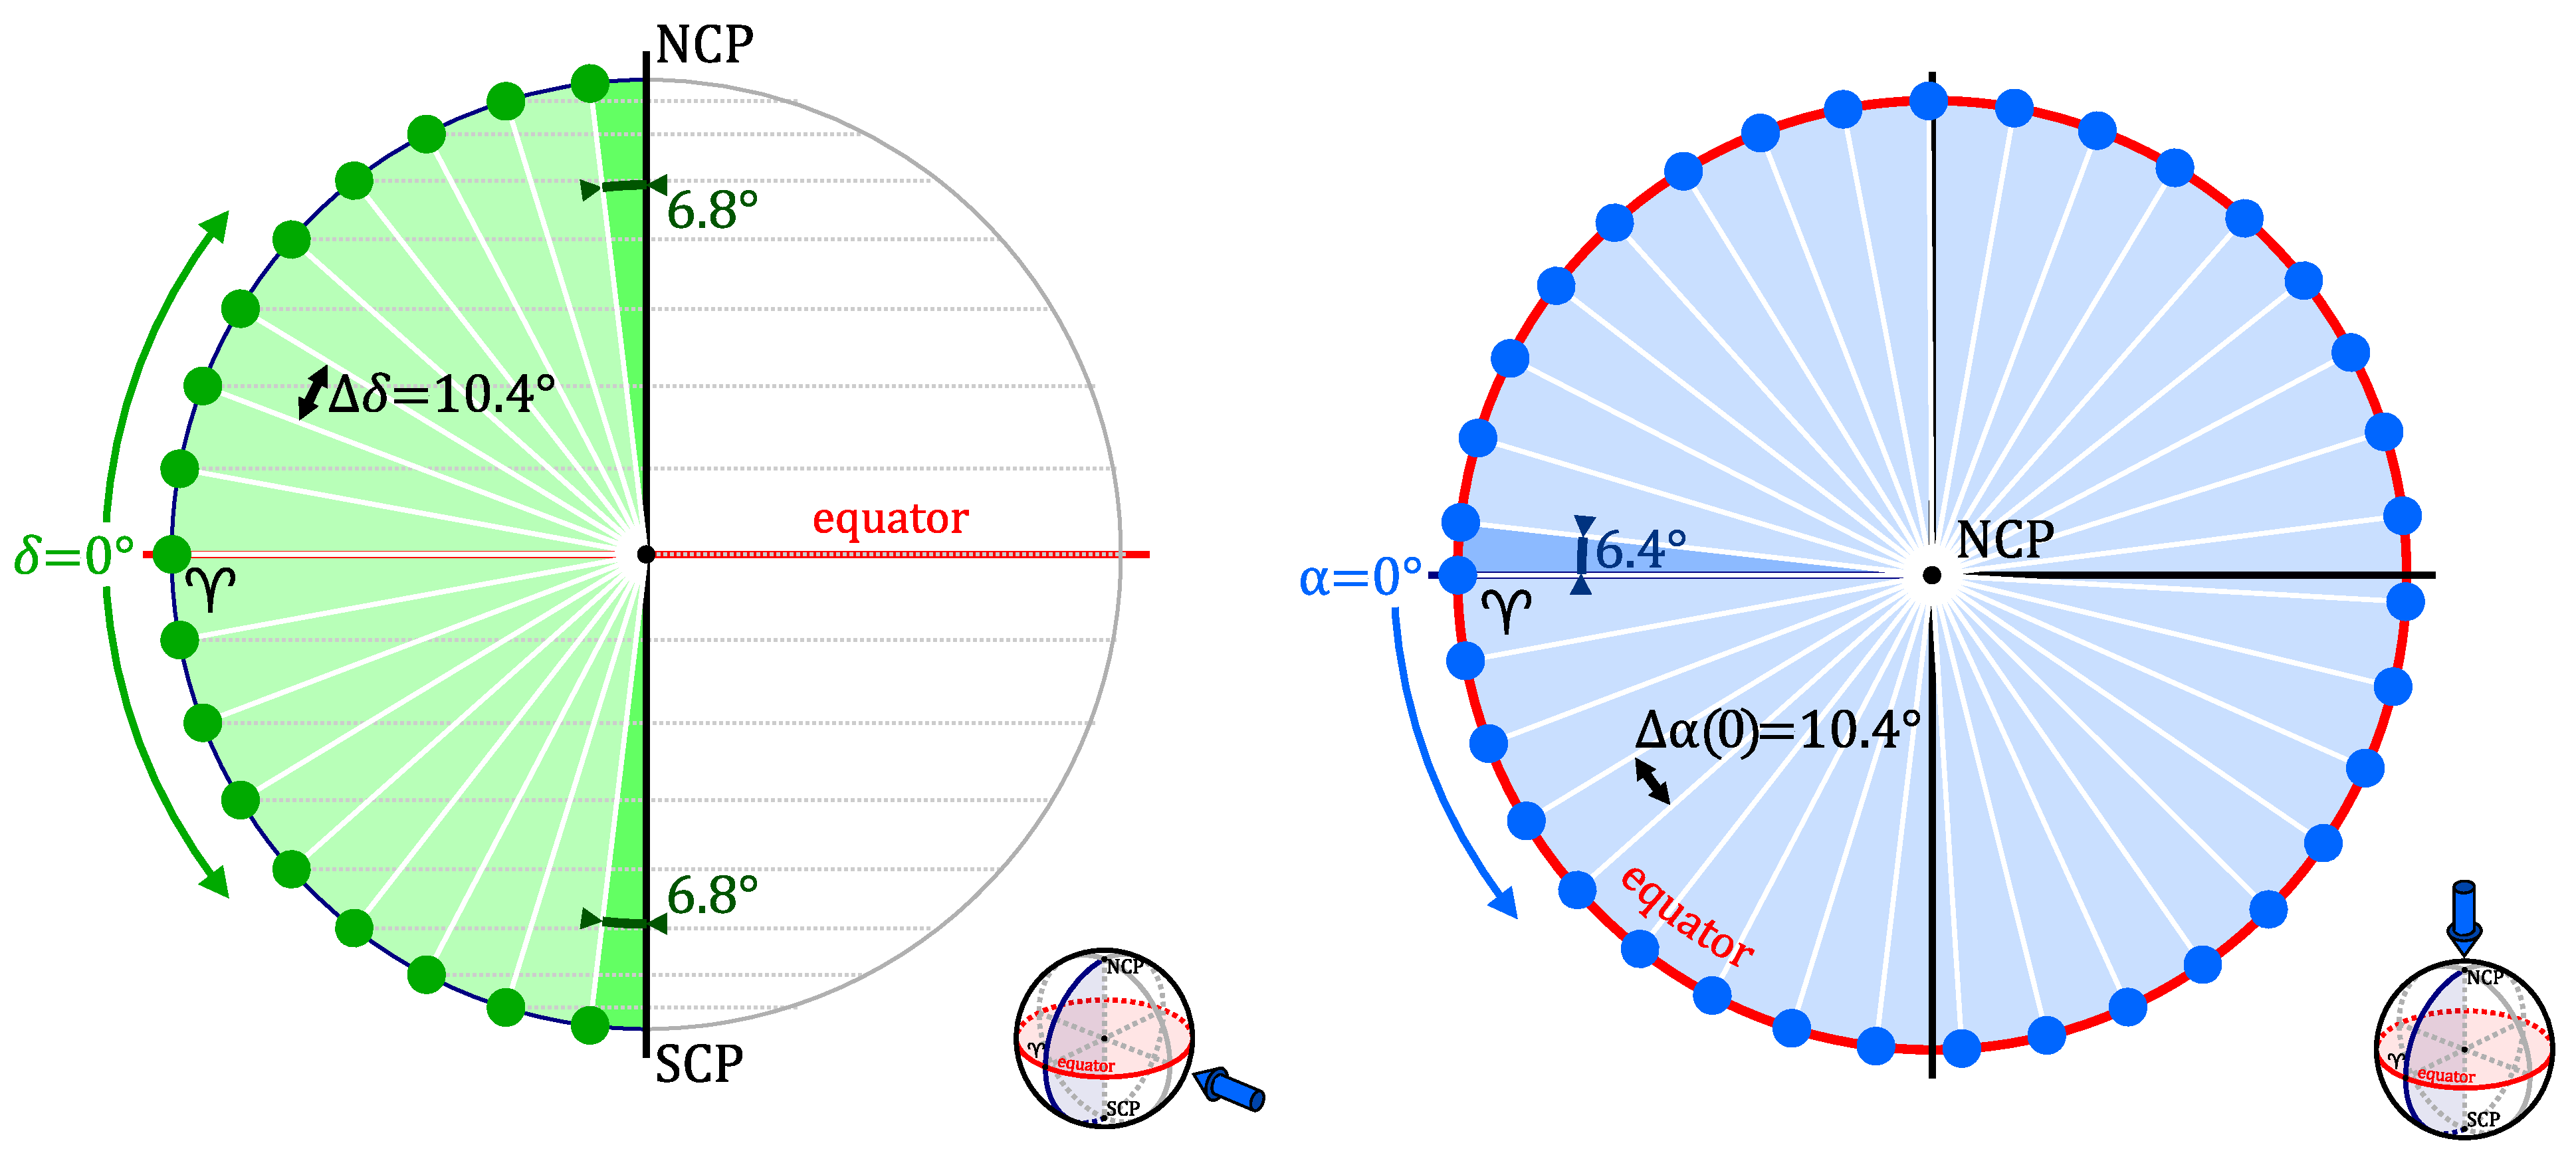
\includegraphics[width=\linewidth]{images/spacing_cosine.pdf}
    \end{center}
    \caption[Tile spacing with the ``cosine'' algorithm]{
        Tile spacing with the ``cosine'' algorithm, with a \SI{13}{\degree}$\times$\SI{13}{\degree} FoV and $0.2$ overlap.
        \\
        \textbf{Left}: \aref{eq:product_deltadelta} gives $\Delta\delta = $ \SI{10.4}{\degree}, which does not divide into \SI{90}{\degree} without a remainder. 17 strips are defined moving away from $\delta=0$, with last being \SI{6.8}{\degree} from the poles. As this is less than half of the field of view (\SI{6.5}{\degree}) the poles themselves will not fall within the area of any tile.
        \\
        \textbf{Right}: \aref{eq:cosine_deltaalpha} gives $\Delta\alpha = $ \SI{10.4}{\degree} on the equator ($\delta=0$). This results in 35 tiles and a reduced spacing of \SI{6.4}{\degree} to the west of the $\alpha=0$ meridian. This remainder will be different for each strip as $\delta$ changes, as visible in \aref{fig:cosine}.
    }\label{fig:cosine_spacing}
\end{figure}

\begin{figure}[p]
    \begin{center}
        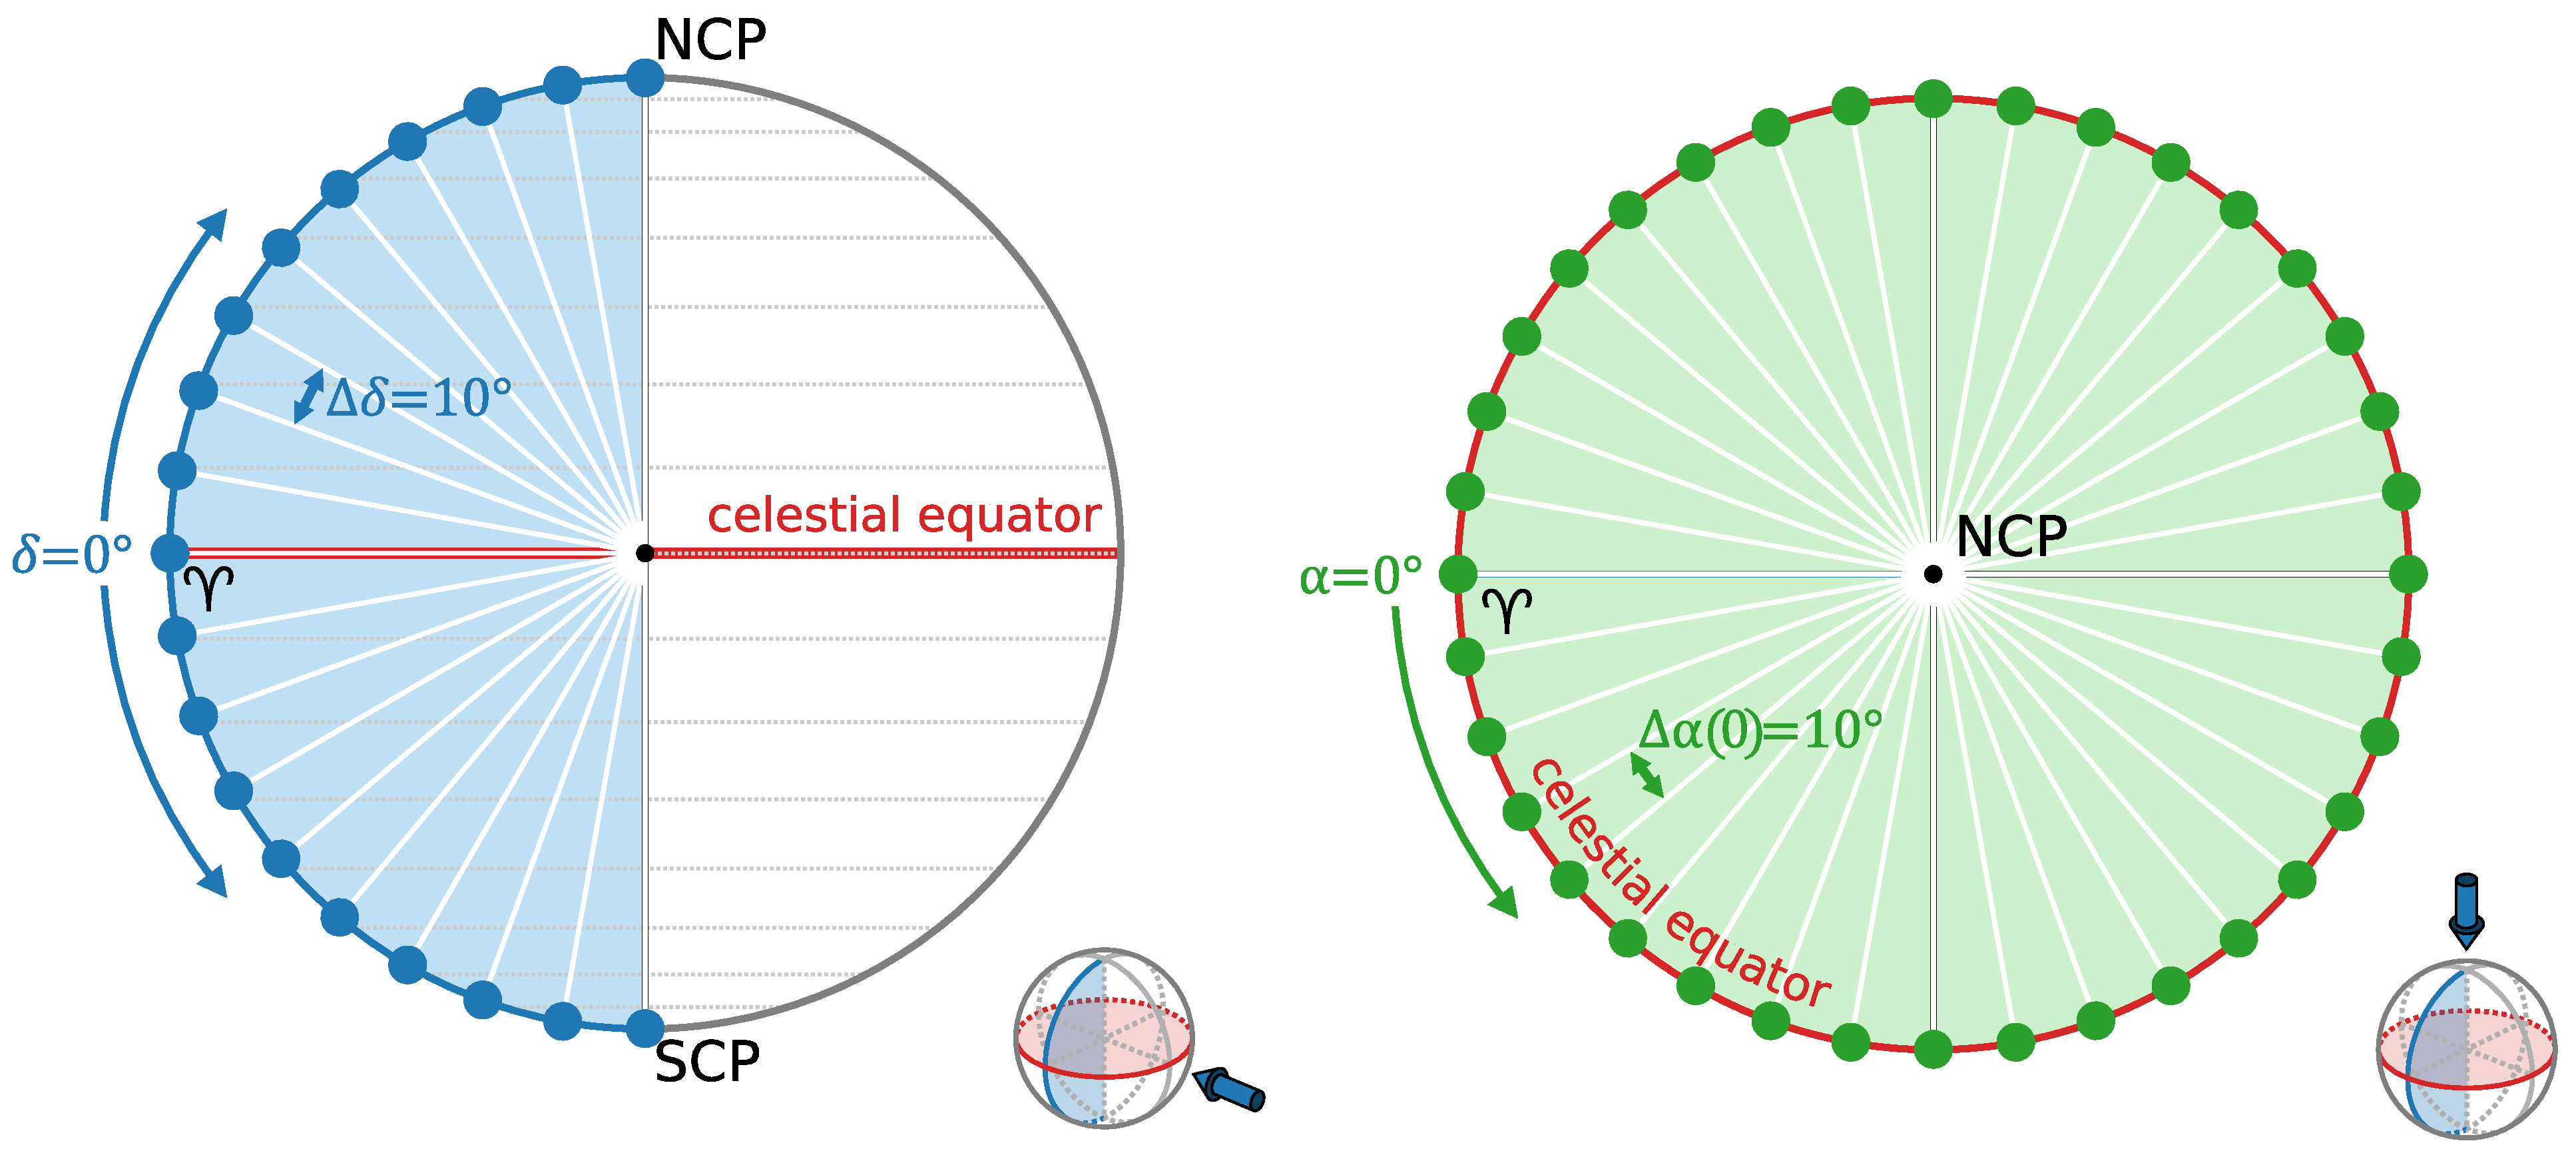
\includegraphics[width=\linewidth]{images/spacing_minverlap.pdf}
    \end{center}
    \caption[Tile spacing with the ``minverlap'' algorithm]{
        Tile spacing with the ``minverlap'' algorithm, with the same parameters as \aref{fig:cosine_spacing}.
        \\
        \textbf{Left:} \aref{eq:minverlap_deltadelta} gives $\Delta\delta = $ \SI{10}{\degree}, therefore neatly arranging 19 strips    between \SI{-90}{\degree} and \SI{90}{\degree}.
        \\
        \textbf{Right:} \aref{eq:minverlap_deltaalpha} also gives $\Delta\alpha = $ \SI{10}{\degree} on the equator ($\delta=0$), so 36 tiles are uniformly arranged around the circumference of the sphere.
    }\label{fig:minverlap_spacing}
\end{figure}

\clearpage

\end{colsection}

% ~~~~~~~~~~~~~~~~~~~~

\subsection{Mapping skymaps to the grid}
\label{sec:mapping_skymaps}
\begin{colsection}

When gravitational wave signals are detected the \gls{lvc} analysis pipelines create HEALPix skymaps to describe the sky localisation, and these are then distributed with the public VOEvent (see \aref{sec:voevents}). GOTO-tile is used to map the skymaps onto the previously-defined sky grid used for the all-sky survey. This requires finding which HEALPix pixels fall within each tile, which is done by defining polygons that match the projected tile areas and using the \pkg{healpy} \code{query\_polygon} function. Then it is simple to sum the probability of these pixels for each tile to give the total probability contained within it. As sky grids might contain overlapping tiles a given pixel may fall within multiple tiles, and therefore contribute to the total probability of more than one tile.

Finding which contour each tile is in is not as simple, and there are multiple ways to define the contour value for the tiles. \aref{fig:sim_skymap_tiles} shows calculating the contained probabilities for tiles using the previous 2D skymap, as well as two methods to calculate the contour values: taking the minimum or the mean of the contained pixel contour values. Using the mean is preferred as it is less susceptible to single outlier pixels.

\aref{fig:170817_gw} shows an example of GOTO-tile applied to the skymap for the GW170817 event \citep{GW170817}. The points within each tile were identified and summed in order to find the total contained probability within each tile. There is some redundancy due to the overlap between tiles, however this is typically negligible (the final GW170817 skymap used was notably smaller than usual LVC skymaps due to the coincident \textit{Fermi} localisation, which makes the overlaps more pronounced).

\begin{figure}[p]
    \begin{center}
        \begin{tabular}{cccccc}
            \multicolumn{3}{c}{Pixel probabilities (from \aref{fig:sim_skymap_probs}):} &
            \multicolumn{3}{c}{Pixel contours (from \aref{fig:sim_skymap_conts}):} \\
            \multicolumn{3}{c}{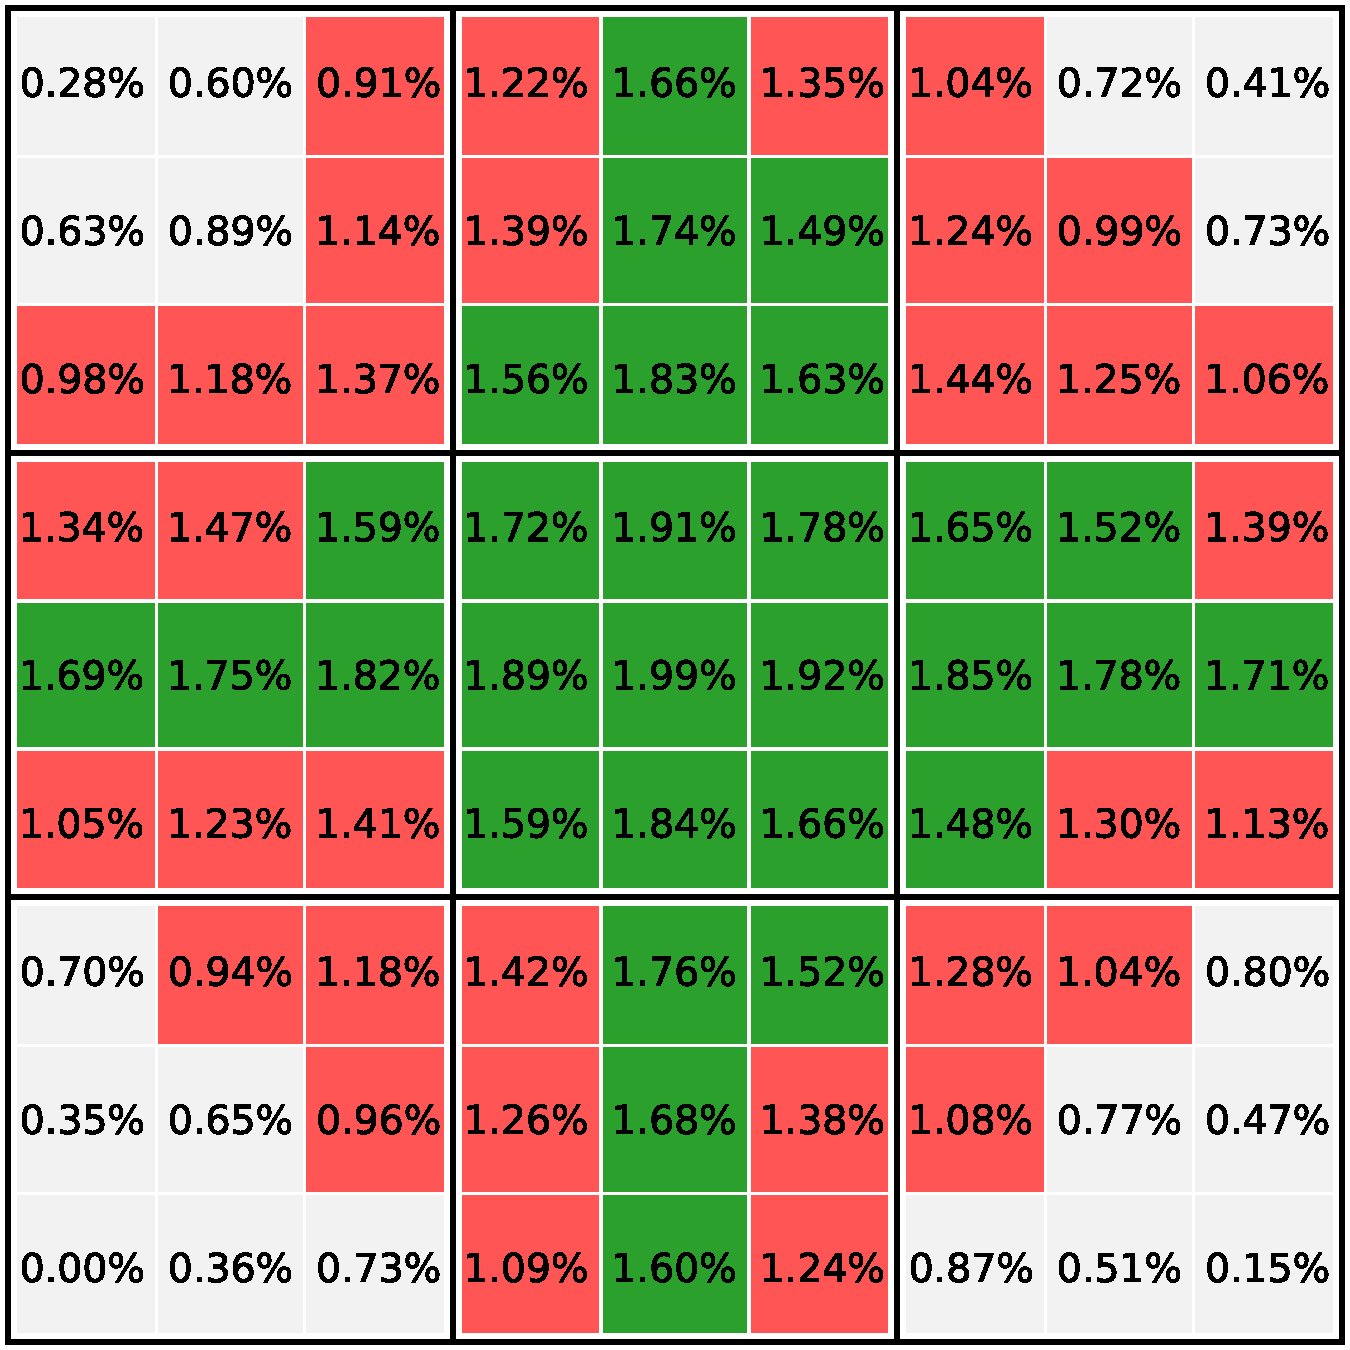
\includegraphics[width=0.46\linewidth]{images/sim/sim_skymap_pix_probs.pdf}} &
            \multicolumn{3}{c}{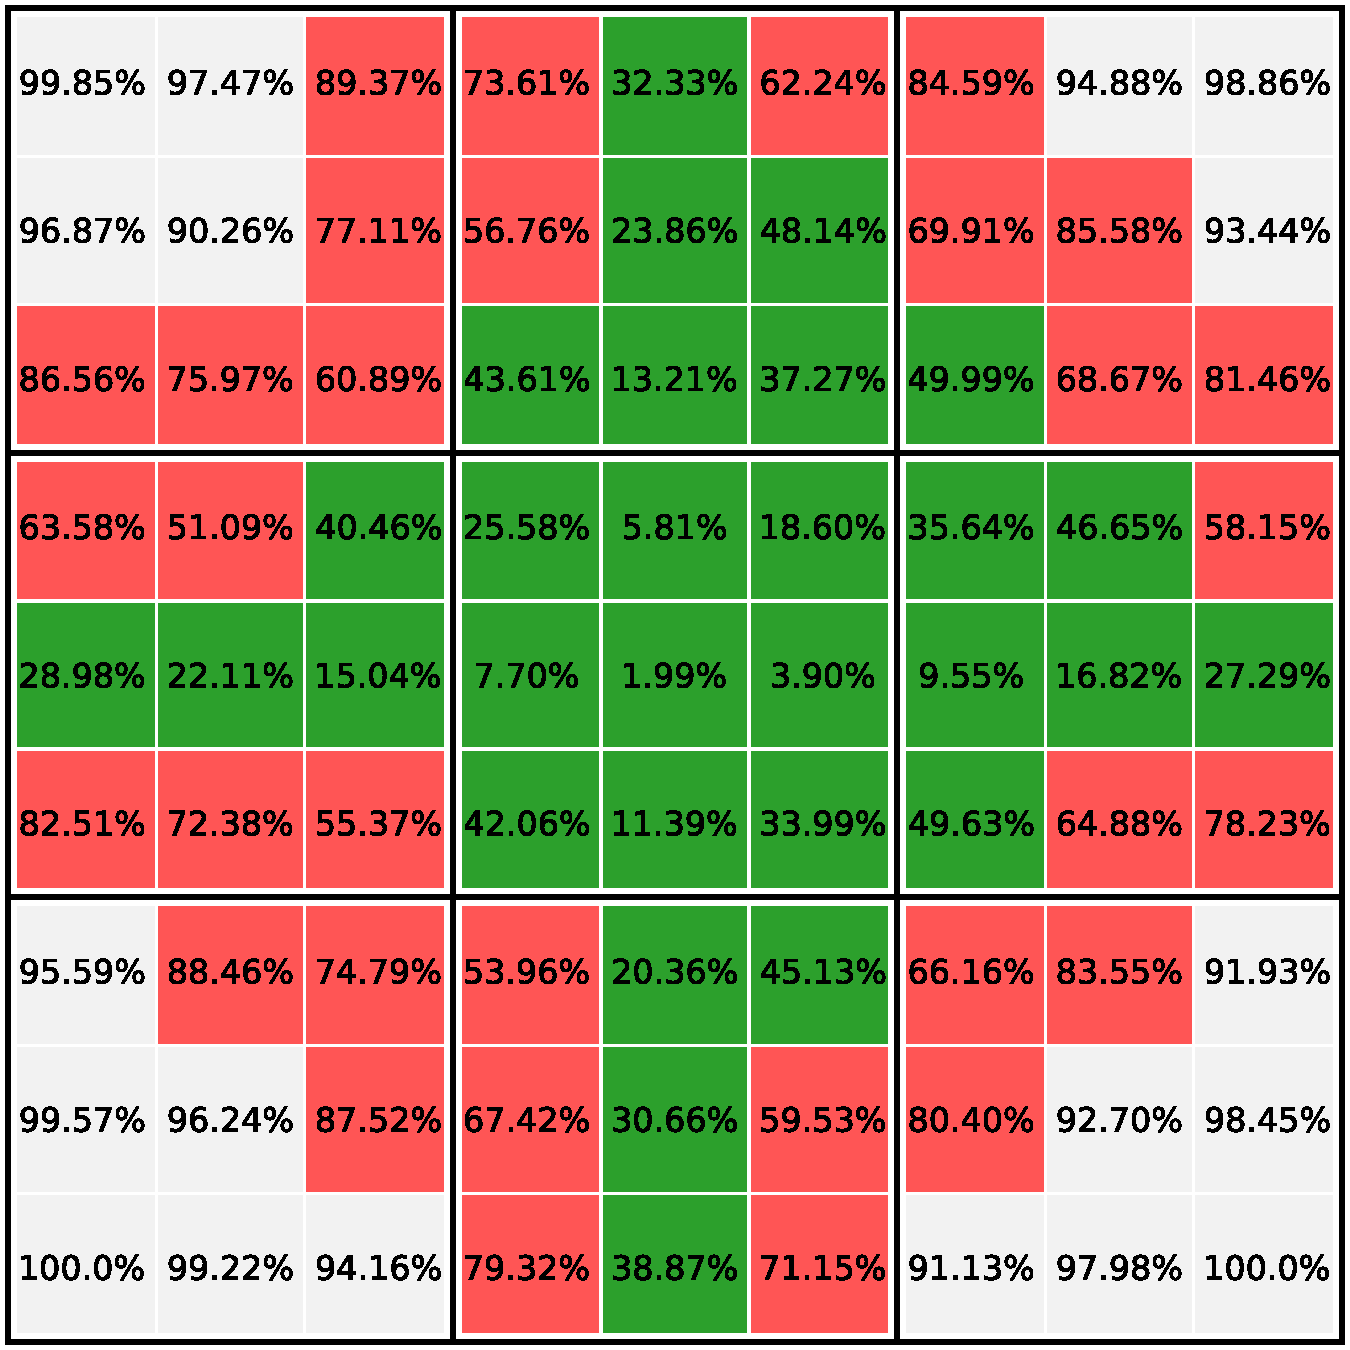
\includegraphics[width=0.46\linewidth]{images/sim/sim_skymap_pix_conts.pdf}} \\
            \multicolumn{2}{c}{Tile contained probabilities:} &
            \multicolumn{2}{c}{Tile minimum contours:} &
            \multicolumn{2}{c}{Tile mean contours:} \\
            \multicolumn{2}{c}{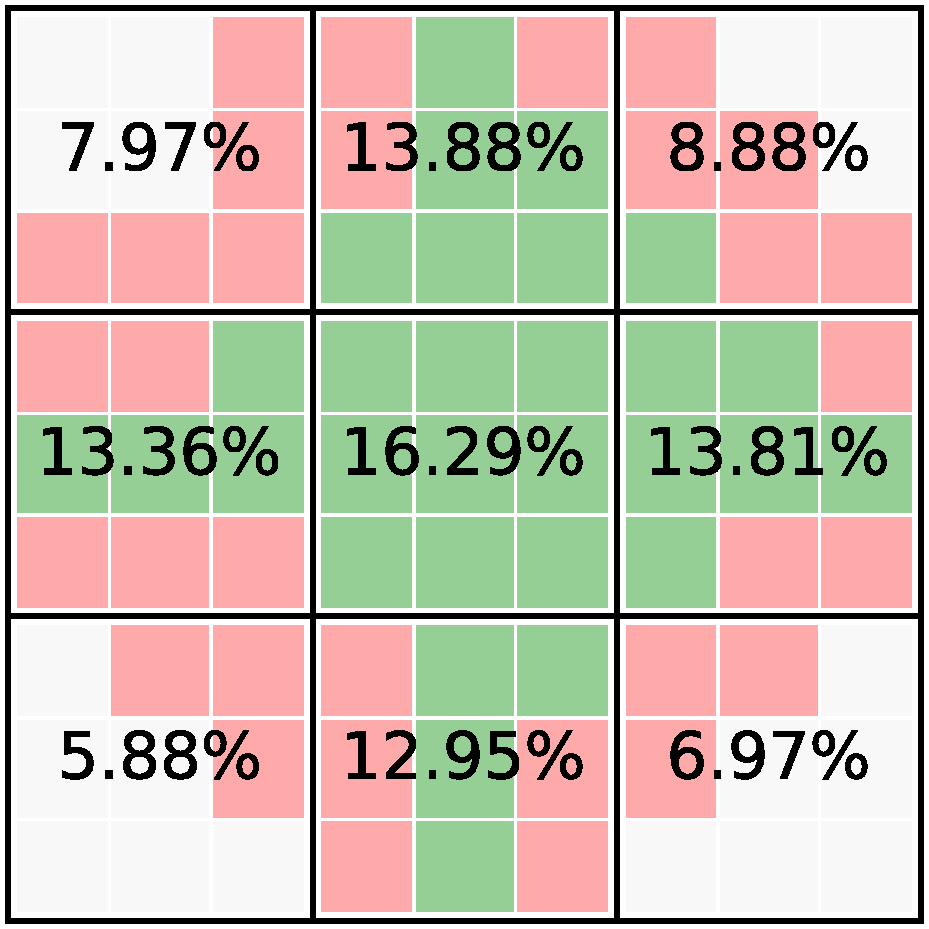
\includegraphics[width=0.3\linewidth]{images/sim/sim_skymap_tile_probs.pdf}} &
            \multicolumn{2}{c}{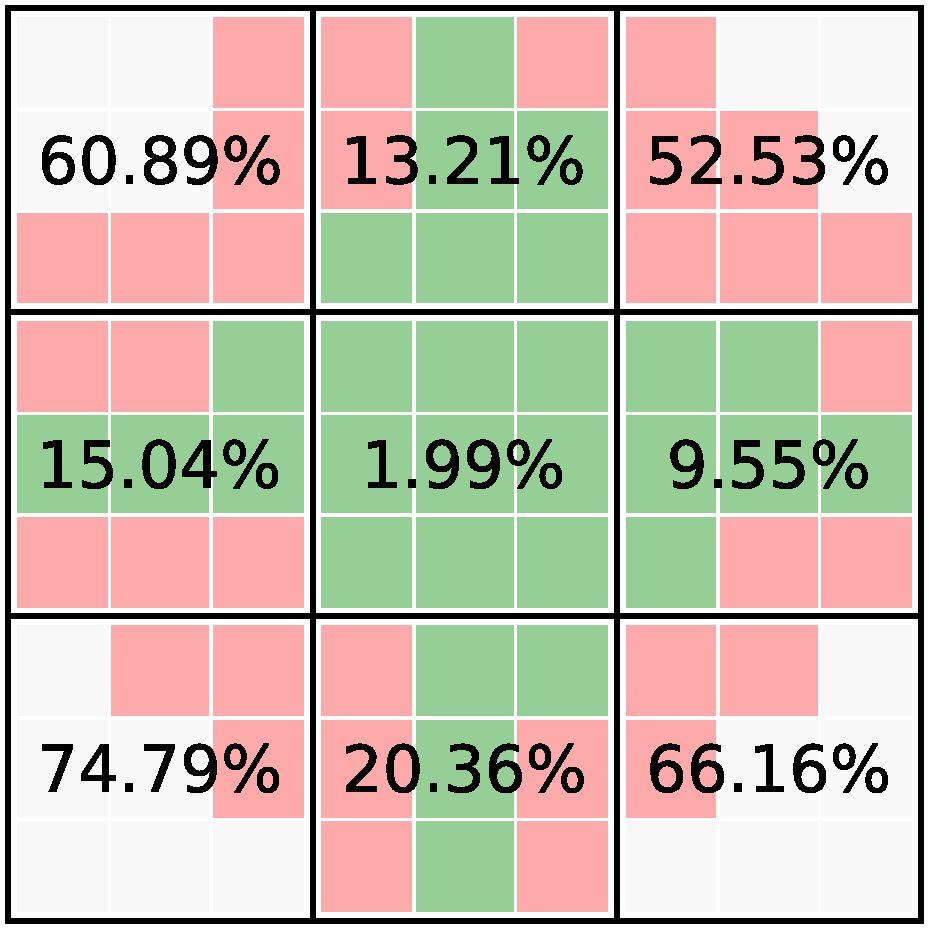
\includegraphics[width=0.3\linewidth]{images/sim/sim_skymap_tile_minconts.pdf}} &
            \multicolumn{2}{c}{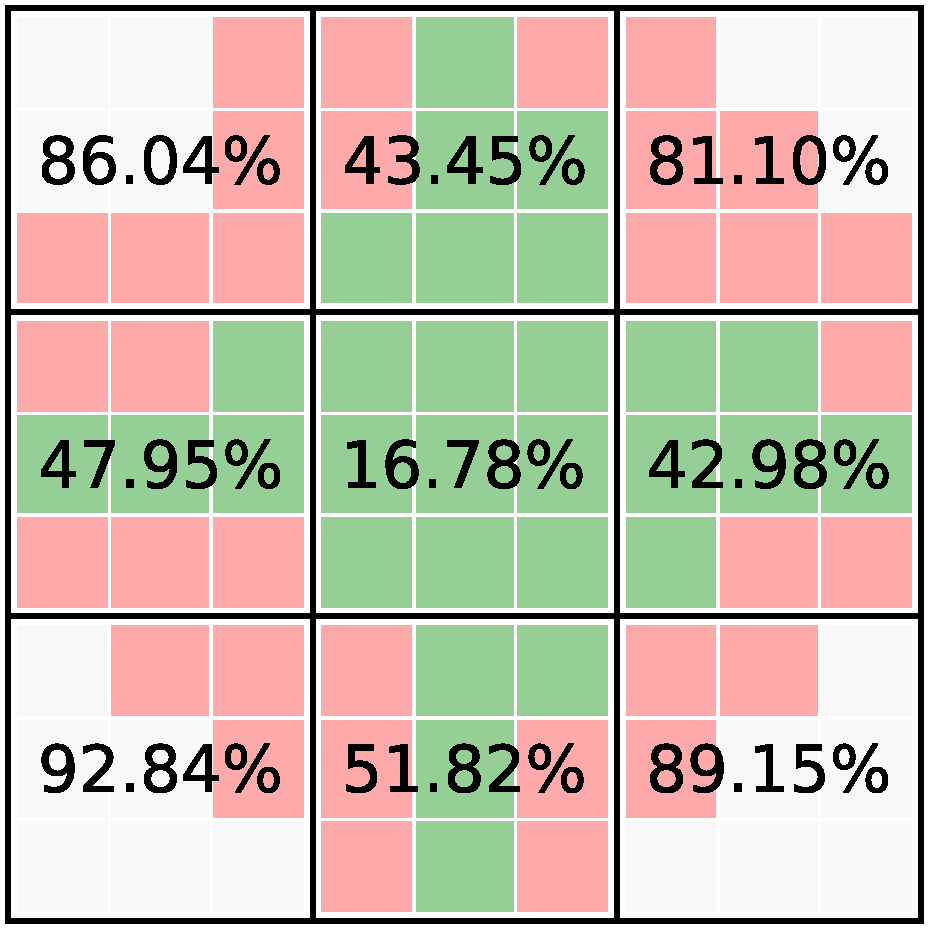
\includegraphics[width=0.3\linewidth]{images/sim/sim_skymap_tile_meanconts.pdf}} \\
        \end{tabular}
    \end{center}
    \caption[Calculating tile probabilities and contours for a 2D skymap]{
        Tiling the same cartoon 2D skymap as \aref{fig:sim_skymap_probs} and \aref{fig:sim_skymap_conts}.\\
        \textbf{Top}: These plots show the pixel probabilities and contour values, coloured with the pixels within the 50\% contour in green and the pixels within the 90\% contour in green or red. The 81 total pixels are divided into 9 tiles, with no overlap for simplicity.\\
        \textbf{Lower-right}: The contained probability within each tile is the sum of the pixel probabilities, in this case each tile contains the sum of the 9 pixels contained within. Overlapping tiles would mean a single pixel might fall within multiple tiles and therefore contribute probability to each.\\
        \textbf{Lower-centre}: One way of finding which contour area each tile is within is to find the minimum contour value of the 9 pixels contained within it. This corresponds to the contour value of the pixel with the highest probability within each tile.\\
        \textbf{Lower-right:} An alternative method is to calculate the mean contour value of the pixels within each tile and use that as the tile contour value. This is less susceptible to single pixels affecting the value than taking the minimum.
    }\label{fig:sim_skymap_tiles}
\end{figure}

\begin{figure}[p]
    \begin{center}
        \includegraphics[width=\linewidth]{images/skymaps_170817_gw.pdf}
    \end{center}
    \caption[Tile probabilities for GW170817]{
        Tile probabilities using the final skymap for GW170817 \citep{GW170817}. The sphere shows the whole skymap for this event, with each pixel coloured by probability, and the location of the source of the event is shown with the blue star. Overlaid is the GOTO-4 sky grid, with tiles of \SI{3.7}{\degree} $\times$ \SI{4.9}{\degree} and overlap of $0.1$. The inset shows the tiles coloured by their contained probability (the sum of all pixels within). The four tiles with contained probability of higher than 5\% are highlighted in red.
    }\label{fig:170817_gw}
\end{figure}

\clearpage

\end{colsection}

% ~~~~~~~~~~~~~~~~~~~~

\end{colsection}

% ########################################

\newpage
\section{Creating skymaps for GRB events}
\label{sec:grb_skymaps}
\begin{colsection}

% ~~~~~~~~~~~~~~~~~~~~

\begin{colsection}

\todo{galaxies here --- go to ``creating custom skymaps''?}

This system described in the previous sections works well for gravitational wave events using \gls{lvc} skymaps, and it has since ben expanded to other types of events. As part of the commissioning observations (\todo{see commissioning}) when the LIGO-Virgo detectors were down \gls{goto} also followed-up \gls{grb} events from the \textit{Fermi} satellite \gls{gbm} \citep{Fermi_GBM}. These events however do not include probability skymaps, instead they only include a central right ascension, declination and error radius. Yik Lun Mong and I developed code in order to create a skymap from these Fermi events, therefore allowing them to be processed by GOTO-tile using the same methods already created for gravitational wave events.

\end{colsection}

% ~~~~~~~~~~~~~~~~~~~~

\subsection{Gaussian skymaps}
\label{sec:gaussian_skymaps}
\begin{colsection}

Instead of loading a skymap from a FITS file, a function was written to create a probability skymap based on a 2D Gaussian profile. First, the error radius ($r$, the 68\% containment radius) is converted into the standard deviation of the distribution $\sigma$ using

\begin{equation}
    \sigma = \frac{r}{\sqrt{2.3}}.
    \label{eq:gaussian_sigma}
\end{equation}

The distance $d$ between a given point on the sphere ($\alpha, \delta$) and the central coordinates of the distribution ($\alpha_c, \delta_c$) is given by

\begin{equation}
    \sin^2 \left ( \frac{1}{2} d \right )
    = \sin^2 \left ( \frac{\delta-\delta_c}{2} \right)
      + \cos (\delta) \cos (\delta_c) \sin^2 \left ( \frac{\alpha-\alpha_c}{2} \right),
    \label{eq:gaussian_distance}
\end{equation}

and the probability at each point is given by

\begin{equation}
    P(\alpha, \delta) = \frac{1}{2\pi\sigma} \exp \left ( \frac{d^2}{2\sigma^2} \right ).
    \label{eq:gaussian_prob}
\end{equation}

In order to create a HEALPix skymap this probability is calculated for every point on the grid, which creates the skymap array. This can then be processed with GOTO-tile exactly like an \gls{lvc} skymap.

Using this above method, skymaps can be created for any single-target alert that has a given error radius. Several sources of transient events, such as \textit{Gaia} or \textit{Swift}, produce very well-localised events with error regions well below the field of view of GOTO, so creating skymaps is less important. The skymaps for \glspl{grb} from \textit{Fermi} however cover much larger areas. For example, the \gls{gbm} detection of GRB~170817A that helped localise the GW170817 gravitational wave detection produced an initial alert with an error radius of \SI{17.45}{\degree}, later reduced to \SI{11.58}{\degree} in the final alert\footnote{GCN Notices available at \url{https://gcn.gsfc.nasa.gov/other/524666471.fermi}}, which corresponded to a 50\% confidence region of $\sim$500~square~degrees \citep{GW170817_Fermi}. The error values given in \gls{gbm} GCN Notices however only account for statistical errors for that event, not systematic errors. The \gls{gbm} systematic errors are described in \citet{Fermi_localisation} to be well modelled by a core Gaussian with a radius of \SI{3.71}{\degree} and a non-Gaussian tail extending to \SI{14}{\degree}. For the purposes of \gls{goto} tiling the tail is ignored, and a single Gaussian is produced with an error radius simply combining the statistical radius ($r_\text{notice}$) and this  systematic profile in quadrature as

\begin{equation}
    r = \sqrt{r_\text{notice}^2 + {(\SI{3.71}{\degree})}^2}.
    \label{eq:fermi_radius}
\end{equation}

This radius is then used with \aref{eq:gaussian_sigma} onwards to create the Gaussian skymap. It should be noted that in reality the probability areas from \textit{Fermi} are not perfectly symmetric Gaussian profiles, but until \gls{gbm} events start being published with \gls{healpix} skymaps this works as a reasonable approximation. For GRB~170817A the skymap and tiling solution is shown in \aref{fig:170817_grb}. Note that the source location falls quite far out of the peak of the \gls{grb} skymap, and had there not been the coincident gravitational wave detection it would be unlikely that the source of the gamma-ray burst would have been observed.

\begin{figure}[p]
    \begin{center}
        \includegraphics[width=\linewidth]{images/skymaps_170817_grb.pdf}
    \end{center}
    \caption[Tile probabilities for GRB 170817A]{
        Tile probabilities using the constructed Gaussian skymap for GRB 170817A \citep{GW170817_Fermi}. As in \aref{fig:170817_gw} the sphere shows the skymap and the GOTO-4 grid, with the identified source of GW170817 shown by the blue star. The tiles highlighted in red each contain more than 1\% of the probability instead of 5\% used in \aref{fig:170817_gw}, due to the greater spread of the skymap meaning no tile here contains more than 5\%.
    }\label{fig:170817_grb}
\end{figure}

\end{colsection}

% ~~~~~~~~~~~~~~~~~~~~

\end{colsection}

% ########################################
